\documentclass[letterpaper,journal]{IEEEtran}
\usepackage{amsmath,amsfonts,amssymb,amsthm}
\usepackage[switch*,mathlines]{lineno}
% IEEEtran builds the title page with a special two-column output routine,
% for which lineno identifies both first-page columns as the right column.
% Keep lines 1--44 (the first column) on the left margin.  Testing the line
% number directly is more robust than testing \c@page with IEEE's title-page
% output routine.
\makeatletter
\let\IEEEorigMakeLineNumberRight\makeLineNumberRight
\renewcommand{\makeLineNumberRight}{%
	\ifnum\c@linenumber<45\relax
		\makeLineNumberLeft
	\else
		\IEEEorigMakeLineNumberRight
	\fi}
\let\makeLineNumberOdd\makeLineNumberRight
\makeatother
\usepackage{textcomp}
\usepackage{url}
\usepackage{graphicx}
\usepackage{cite}
\usepackage{xcolor}
% Keep all line numbers black, including beside highlighted revisions.
\let\OriginalLineNumberFont\linenumberfont
\renewcommand{\linenumberfont}{\OriginalLineNumberFont\color{black}}
\usepackage{mathrsfs}
\usepackage{booktabs}
\usepackage{tabularx}
\usepackage{tikz}
\usetikzlibrary{arrows.meta,positioning,calc}

\hyphenation{op-tical net-works semi-conduc-tor IEEE-Xplore}

% Define theorems as they are not default in IEEEtran
\newtheorem{remark}{Remark}[section]
\newtheorem{theorem}{Theorem}[section]
\newtheorem{lemma}{Lemma}[section]
\newtheorem{corollary}{Corollary}[section]

\begin{document}
	\bstctlcite{IEEEexample:BSTcontrol}
		
	
	\title{Analyzing the Impact of Rumor Fatigue and Delay Effects on Information Propagation Dynamics via TransPINN}
	
	\author{Deliang Li, Yi Zhao, and Yifeng Wang
		\thanks{This work was supported by the National Natural Science Foundation of China (NSFC) under Project No. 62473115 and the Fundamental Research Plan of Shenzhen Government under Project No. JCYJ20240813105202004.}
		\thanks{The authors are with the School of Science, Harbin Institute of Technology, Shenzhen, China. (Corresponding author: Yi Zhao).}}
	
	% The paper headers
	\markboth{IEEE Transactions on Computational Social Systems}%
	{Li \MakeLowercase{\textit{et al.}}: Analyzing the Impact of Rumor Fatigue and Delay Effects}
	
	\maketitle
	\linenumbers
	
	\begin{abstract}
		Rumor spreading on social media is affected by information delays, media intervention, and changes in user attention. 
		We propose a time-delayed rumor model that separates information exposure from active cognitive processing. 
		The model includes competing corrective and rumor-inciting media. 
		It also uses a Holling-II fatigue term to describe the reduced user response caused by information overload. 
		We prove that the model is well posed and derive the rumor propagation threshold. 
		We then analyze system stability and delay-induced oscillations. 
		To estimate unknown parameters and hidden states from sparse data, 
		we develop a Transformer-based physics-informed neural network called TransPINN. 
		Its self-attention mechanism helps capture the long-range temporal dependence created by the delay. 
		\textcolor{red}{We test TransPINN on four real rumor events: Hurricane Harvey, CSDC-Rumor, the Ottawa shooting, and the Sydney cafe siege. Under the same data splits and training budget, we compare it with PINN, LSTM-PINN, causal TimePINN, and a parameter-matched model without attention. Within this comparison, TransPINN achieves the lowest NRMSE.  } 
		The numerical results also show that delays can shift the rumor peak and cause secondary oscillations. Cognitive fatigue reduces the peak under information overload. Finally, we formulate an optimal control strategy that reduces rumor activity while limiting intervention costs.
	\end{abstract}
	
	\begin{IEEEkeywords}
		Rumor dynamics, delay differential equations, TransPINN, cognitive fatigue, identifiability, optimal control.
	\end{IEEEkeywords}
	
	\section{Introduction}
	\IEEEPARstart{W}{ith} the widespread adoption of social media platforms, rumors can propagate rapidly through instant communication networks, posing significant threats to public cognition\cite{shen2024cognitive}, social order\cite{xia2007emergence}, and public safety\cite{knapp1944psychology,lv2022new,dong2025rumor,mou2022social,li2024information,xiao2022diffusion,zhong2023rumor,jiang2022rumor}. Such propagation distorts public judgment and induces social panic, while simultaneously undermining the foundations of public trust. In the digital era, rumor diffusion exhibits distinct characteristics, including accelerated transmission, expanded reach, and amplified societal impact, enabling rumors to achieve viral-like replication within remarkably short time spans.
	
	Owing to the strong analogy between rumor propagation and epidemic transmission, early research endeavors modeled rumor diffusion using mathematical frameworks originally developed for infectious diseases. In the 1960s, Daley and Kendall \cite{daley1964epidemics} proposed the classical D–K model, which categorizes individuals into ignorants, spreaders, and stiflers. Subsequently, Maki and Thompson \cite{maki1973mathematical,gani2000maki} refined this paradigm through the M–T model, thereby further advancing the theoretical foundations of rumor-spreading dynamics.
	In realistic communication environments, time-delay effects are inherent throughout the rumor life cycle, encompassing information generation, dissemination, intervention, and eventual dissipation. To capture such effects, Fu et al.\cite{fu2025rumor} developed a rumor-spreading model incorporating three identical time delays, aiming to examine the influence of uniform decision-making and response delays across multiple transition processes. Building upon this uniform-delay framework, Wei et al. \cite{wei2025stability} introduced two distinct time delays into the transitions from ignorants to spreaders and from spreaders to stiflers, respectively, while also incorporating a saturation effect to account for heterogeneous response lags and bounded contact rates. Further extending this line of research, Sheng et al.\cite{sheng2025asymptotic} integrated three time delays together with two saturation functions, investigating the combined influence of multiple delay mechanisms and nonlinear incidence rates on the asymptotic stability of rumor-spreading dynamics.
	In parallel, the stochastic-systems literature has developed rigorous stability and synchronization criteria for mixed time-delay systems under aperiodic intermittent control, regime-switching diffusion, and stochastic hybrid impulses \cite{zhang2025semiglobal,zhang2025exponential,zhang2022stability}.
	
	\textcolor{red}{
		Holling-II responses have previously represented bounded contact or attention in rumor models \cite{huo2016holling,huo2020stochastic}. In the present model, the decreasing factor is used only as a phenomenological description of reduced response under information overload. Recent empirical work likewise emphasizes that overload, uncertainty, and repeated exposure can change participation and diffusion patterns \cite{huang2026landscape,he2026uncertainty}.	
	}

	\textcolor{red}{
	Physics-informed neural networks (PINNs) offer a way to combine differential-equation constraints with irregular observations. Specific DDE solvers based on PINNs have been proposed \cite{he2025ddepinn,yao2026ddepinn}, while PINNsFormer uses self-attention to propagate temporal information across pseudo-sequences \cite{zhao2024pinnsformer}. Physics-informed LSTM networks provide a recurrent baseline \cite{zhang2020phylstm}, and causal residual weighting supplies a time-ordered PINN baseline \cite{wang2024causalpinn}. Other recent scientific-learning architectures use auxiliary outputs, Hermite interpolation, Kolmogorov--Arnold networks, or wavelets \cite{saini2026apinn,kumar2026hermite,kumar2026kan,kumar2026wavelet}. These methods motivate comparisons, but they do not by themselves solve the measurement and identifiability difficulties of a partially observed rumor model.
	}

	\textcolor{red}{
	The contribution of this paper is therefore deliberately limited to four elements. First, a survival-weighted exposure cohort replaces the non-positive delayed-stock outflow used in an earlier formulation. Second, the resulting renewal structure yields an explicit delay-dependent threshold and a compact characteristic equation for critical-delay analysis. Third, TransPINN is formulated with the same history operator and with an explicit activity-measurement model. Fourth, a four-scenario, chronological forecasting study compares TransPINN with a standard MLP-PINN, LSTM-PINN, causal TimePINN, and an exactly parameter-matched no-attention ablation. To further assess the effects of model size and training budget, a supplementary experiment compares models with matched parameter counts and update budgets, including a data-only Transformer as an additional baseline. The evaluation distinguishes robustness across random seeds from forecasting performance obtained through validation-based model selection. The positivity proof, next-generation argument, Hopf test, and Pontryagin principle are standard tools. The novelty lies in their consistent application to a partially observed forecasting problem incorporating cohort delays, antagonistic media, and fatigue.
	}

	\textcolor{red}{
	The empirical component combines the processed Hurricane Harvey activity table \cite{jiang2021reciprocal}, the THUNLP CSDC-Rumor archive \cite{csdc2021rumor}, and stance-annotated Ottawa and Sydney conversations from RumourEval \cite{zubiaga2016threads,gorrell2019rumoureval,rumoureval2019data}. These sources do not share an identical observation mechanism. We therefore model harmonized rumor/corrective activity fluxes, retain event-specific reporting scales, and treat the CSDC corrective series as a fact-check proxy rather than an individual stance label. No spline point is treated as a new observation, and no neural variability band is called a confidence interval.
	}

	The paper is organized as follows. Section~\ref{sec1} defines the delay model and notation. Section~\ref{sec2} establishes positivity, the reproduction threshold, and the critical-delay conditions. Section~\ref{sec3} specifies the observation operator and reports the four-scenario baseline, ablation study, and follow-up robustness grid. Section~\ref{sec4} gives the corrected optimal-control conditions. Section~\ref{sec5} summarizes the supported conclusions and limitations.
	
	\section{Rumor Propagation Model Formulation and Dynamic Transitions}
	\label{sec1}
	
	In this section, we establish the theoretical framework for the time-delayed rumor propagation model, designed to capture the interplay between cognitive latency and antagonistic media environments. We delineate the population stratification and the dynamic transmission mechanisms, explicitly incorporating Holling-II type cognitive fatigue and competitive inhibition functions to reflect real-world psychological constraints. The governing system of delay differential equations is derived to quantify these nonlinear interactions. This mathematical formulation serves as the fundamental basis for the dynamical stability analysis and the data-driven parameter identification presented in the subsequent sections.
	
	\subsection{\textcolor{red}{States assumptions}}
	\textcolor{red}{
	The human population is divided into seven mutually exclusive states: susceptible users without and with verification ability ($S_u,S_e$), passively exposed users ($E$), users actively deliberating ($H$), rumor spreaders ($R$), debunkers ($D$), and withdrawn users ($U$). The two dimensionless media intensities fix meanings throughout: $M_1$ is corrective media and $M_2$ is rumor-inciting media. A fraction $\lambda$ of recruitment enters $S_e$ and the remaining fraction enters $S_u$. Each short empirical cascade is modeled as a closed normalized event cohort, so $\Lambda=d_h=0$ and $N(0)=1$. The open-population terms are retained only for the general analysis.
	}

	\begin{figure*}[t]
		\centering
		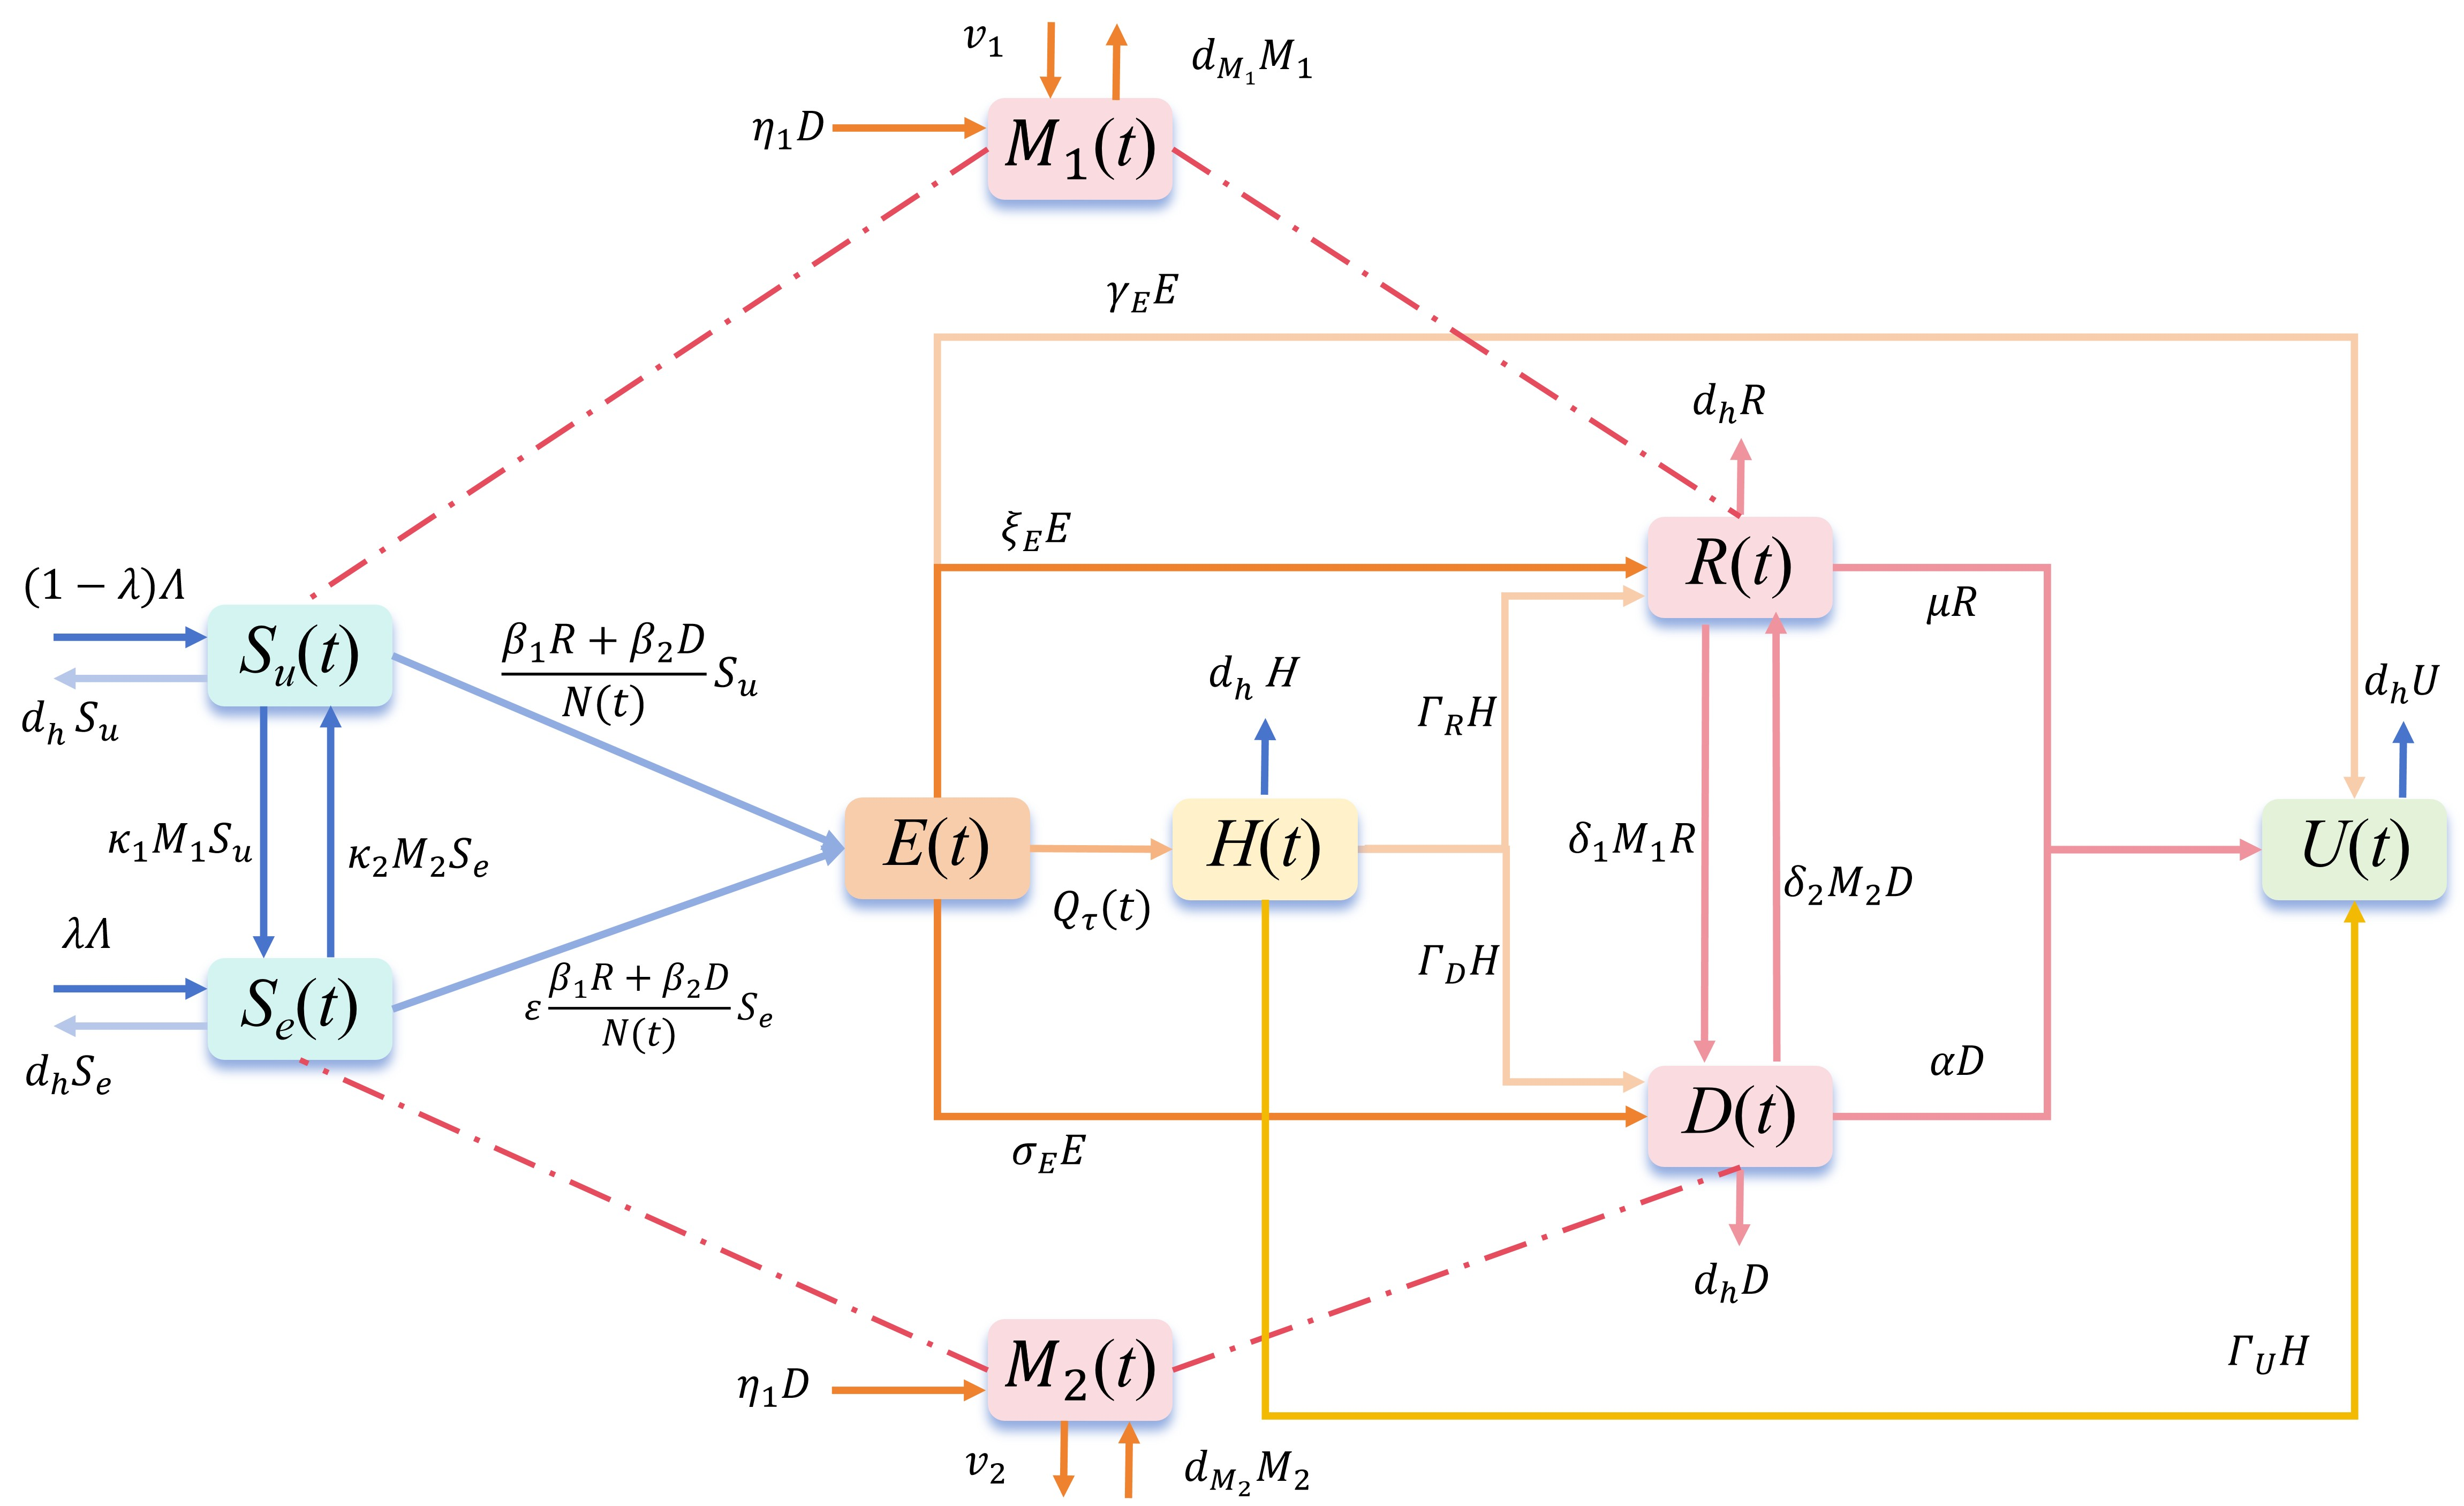
\includegraphics[width=1.0\textwidth]{1gainiantu.jpg}
		\caption{Rumor–media model with noncrossing flow paths. The main \(E\to H\to U\) path is straight, while direct exits from \(E\) and \(R\leftrightarrow D\) transitions follow separate routes. Repeated \(U\) nodes represent the same withdrawal compartment. The delayed \(E\to H\) transition is governed by the survival-weighted cohort flux \(Q_\tau(t)\), defined in Eq.~\eqref{eq:cohort_flux}.}
		\label{fig-1}
	\end{figure*}

	\textcolor{red}{
	The distinction between \(E\) and \(H\) is defined in terms of their respective roles in the model. State $E$ records passive exposure, whereas $H$ records active evaluation. The fixed delay $\tau$ is the time, measured in hours, from a new exposure to completion of the passive-processing stage. Media at the exposure time determine the fraction entering this pathway. Users who leave $E$ through other routes before $\tau$ do not subsequently enter $H$.
	}

	\subsection{\textcolor{red}{Survival-weighted delay model}}
	Define the new-exposure incidence and a bounded pathway-selection probability by
	\begin{align}
		\mathcal I(t)&=(\beta_1R(t)+\beta_2D(t))\frac{S_u(t)+\varepsilon S_e(t)}{N(t)},\label{eq:incidence}\\
		p(t)&=\frac{\rho M_1(t)M_2(t)}{1+\rho M_1(t)M_2(t)}\in[0,1),\label{eq:path_probability}\\
		a_E&=\xi_E+\sigma_E+\gamma_E+d_h.
	\end{align}
	The completed-processing flux is
	\begin{equation}
		\textcolor{red}{Q_\tau(t)=p(t-\tau)\mathcal I(t-\tau)e^{-a_E\tau}.}
		\label{eq:cohort_flux}
	\end{equation}
	\textcolor{red}{Thus, $\mathcal I(t-\tau)$ is the cohort exposed $\tau$ hours earlier, $p(t-\tau)$ is the fraction assigned to active processing at that exposure time, and $e^{-a_E\tau}$ is the probability that an individual in this cohort remains in $E$ throughout the delay interval without leaving through any of the competing exit pathways.
	If the network time is scaled to $s=(t-t_0)/(t_f-t_0)$, the delay supplied to the network is $\tau_s=\tau/(t_f-t_0)$.}
	\textcolor{red}{The governing system is}
	\begin{equation}
		\label{equ_1}
		\left\{
		\begin{aligned}
		\dot S_u={}&(1-\lambda)\Lambda-d_hS_u-\kappa_1M_1S_u+\kappa_2M_2S_e\\
		&-\beta_1RS_u/N-\beta_2DS_u/N,\\
		\dot S_e={}&\lambda\Lambda-d_hS_e+\kappa_1M_1S_u-\kappa_2M_2S_e\\
		&-\varepsilon\beta_1RS_e/N-\varepsilon\beta_2DS_e/N,\\
		\dot E={}&\mathcal I(t)-a_EE-Q_\tau(t),\\
		\dot H={}&Q_\tau(t)-(\Gamma_R+\Gamma_D+\Gamma_U+d_h)H,\\
		\dot R={}&\xi_EE+\Gamma_RH-(\mu+d_h+\delta_1M_1)R+\delta_2M_2D,\\
		\dot D={}&\sigma_EE+\Gamma_DH+\delta_1M_1R-(\alpha+d_h+\delta_2M_2)D,\\
		\dot U={}&\gamma_EE+\mu R+\alpha D+\Gamma_UH-d_hU,\\
		\dot M_1={}&\eta_1D+v_1-d_{M_1}M_1,\\
		\dot M_2={}&\eta_2R+v_2-d_{M_2}M_2.
		\end{aligned}\right.
	\end{equation}
	Here $N=S_u+S_e+E+H+R+D+U$. The media variables are dimensionless indices, and their decay rates $d_{M_i}$ are distinct from human exit $d_h$.

	The media-driven rates are defined consistently with Fig.~\ref{fig-1}:
	
	\begin{equation}
		\textcolor{red}{
		\label{sys:functions}
		\begin{aligned}
		\Gamma_R(M)&=q_R\frac{M_2}{1+\varpi_1M_1}\frac{\chi}{\chi+M_1+M_2},\\
		\Gamma_D(M)&=q_D\frac{M_1}{1+\varpi_2M_2}\frac{\chi}{\chi+M_1+M_2},\\
		\Gamma_U(M)&=q_U\frac{M_1+M_2}{\chi+M_1+M_2}.
		\end{aligned}}
	\end{equation}
	
	\textcolor{red}{Consequently, $\varpi_1$ measures how strongly corrective media inhibit $H\to R$, while $\varpi_2$ measures how strongly rumor media inhibit $H\to D$. Increasing $\varpi_1$ cannot increase $\Gamma_R$, and increasing $\varpi_2$ cannot increase $\Gamma_D$. The factor $\chi/(\chi+M_1+M_2)$ decreases with total information load. The parameters \(q_R,q_D,q_U\) are baseline transition rates, measured in \(\mathrm{h}^{-1}\). }

	Table~\ref{tab:parameters} summarizes the model parameters and their inferential roles. Time is measured in hours in the analytical model and is normalized to each observed event horizon in Section~\ref{sec3}. $M_i$ are dimensionless. In the table, F denotes quantities fixed by design or normalization, whereas G denotes quantities that may be confounded in the full inverse problem. These labels do not assert identifiability. Section~\ref{sec:identifiability} summarizes the identifiability results. Complete empirical settings, fitted values, and conditional intervals are provided in Supplementary Material.

	\begin{table*}[t]
		\caption{\textcolor{red}{Model parameters and inferential role}}
		\label{tab:parameters}
		\centering\scriptsize
		\begin{tabularx}{\textwidth}{@{}lXllXl@{}}
		\toprule
		Symbol & Meaning & Unit/role & Symbol & Meaning & Unit/role\\
		\midrule
		$\Lambda$ & recruitment into the event cohort & proportion h$^{-1}$, F & $\lambda$ & fraction recruited to $S_e$ & 1, F\\
		$d_h$ & human exit/churn rate & h$^{-1}$, F & $\beta_1,\beta_2$ & exposure rates due to $R,D$ & h$^{-1}$, G\\
		$\varepsilon$ & relative exposure of $S_e$ & 1, F & $\kappa_1,\kappa_2$ & media-driven $S_u\leftrightarrow S_e$ rates & h$^{-1}$, G\\
		$\xi_E,\sigma_E$ & direct $E\to R,D$ rates & h$^{-1}$, G & $\gamma_E$ & direct $E\to U$ rate & h$^{-1}$, G\\
		$\rho$ & scale in the bounded pathway gate $p$ & 1, G & $\tau$ & cognitive-processing delay & h, G\\
		$q_R,q_D,q_U$ & baseline $H\to R,D,U$ rates & h$^{-1}$, G & $\chi$ & fatigue tolerance threshold & media unit, G\\
		$\varpi_1$ & corrective inhibition of $H\to R$ & 1, G & $\varpi_2$ & rumor inhibition of $H\to D$ & 1, G\\
		$\mu,\alpha$ & withdrawal rates from $R,D$ & h$^{-1}$, G & $\delta_1,\delta_2$ & $R\leftrightarrow D$ media conversion rates & h$^{-1}$, G\\
		$\eta_1,\eta_2$ & endogenous media-generation rates & h$^{-1}$, G & $v_1,v_2$ & exogenous media input & media h$^{-1}$, F/G\\
		$d_{M_1},d_{M_2}$ & decay rates of the two media indices & h$^{-1}$, G & $N$ & event-cohort normalization & proportion, F\\
		\bottomrule
		\end{tabularx}
	\end{table*}

	\textcolor{red}{A delay differential equation (DDE) requires a history function specifying the system state over the interval $[-\tau,0]$, rather than only an initial value at $t=0$. We assume a continuous, nonnegative history function $\phi\in C([-\tau,0],\mathbb R_+^9)$ and compute $\mathcal I(s)$ and $p(s)$ from $\phi(s)$ for $s\in[-\tau,0]$. The prescribed history is compatible with the exposure-cohort structure if}
	\begin{equation}
		\textcolor{red}{
		E(0)\geq\int_{-\tau}^{0}e^{a_Es}p(s)\mathcal I(s)\,ds.
		\label{sys:init}}
	\end{equation}
	\textcolor{red}{
	This condition ensures that $E(0)$ is sufficient to include all surviving members of pre-observation cohorts scheduled to complete processing after $t=0$.
	}
	

	\section{\textcolor{red}{Dynamical Analysis of the Model}}
	\label{sec2}

	\begin{table*}[t]
		\caption{\textcolor{red}{Theoretical scope relative to delayed rumor models}}
		\label{tab:theory_comparison}
		\centering\footnotesize
		\begin{tabularx}{\textwidth}{@{}lXX@{}}
		\toprule
		Result & Refs.~\cite{fu2025rumor,wei2025stability,sheng2025asymptotic} and related control work \cite{belhdid2024optimal} & Present formulation\\
		\midrule
		Positivity & Standard quasipositivity for delayed compartment models & Cohort representation and the explicit compatibility inequality \eqref{sys:init}. No delayed stock is subtracted from $E(t)$\\
		Threshold & Next-generation calculations for prescribed delay structures & Renewal calculation with the survival probability $e^{-a_E\tau}$ and both $R$ and $D$ activity pathways\\
		Delay stability & Characteristic-root and Hopf methods for delayed rumor systems & Compact characteristic equation for the cohort delay and antagonistic $R$--$D$ conversion\\
		Control & Standard Pontryagin and forward--backward sweep methods & Complete fatigue derivatives for rumor suppression and corrective-media promotion\\
		Inverse problem & Generally not considered in the cited analytical models & History-aware observation model, exact media-scale non-identifiability proof, and conditional sensitivity/profile analysis\\
		\bottomrule
		\end{tabularx}
	\end{table*}

	\subsection{Well-posedness and positive invariance}
	\begin{theorem}[Positivity and boundedness]
		\label{thm:positive}
		\textcolor{red}{Suppose all parameters are nonnegative, $0\leq\lambda,\varepsilon\leq1$, and the history is continuous, nonnegative, and satisfies \eqref{sys:init}. System~\eqref{equ_1} has a unique nonnegative solution. If $d_h>0$, then}
		\textcolor{red}{		
		\begin{align*}
		N(t)&\leq N_{\max}:=\max\{N(0),\Lambda/d_h\},\\
		M_i(t)&\leq\max\{M_i(0),(\eta_iN_{\max}+v_i)/d_{M_i}\},\quad i=1,2.
		\end{align*}
		}
		\textcolor{red}{
		For the closed event model ($\Lambda=d_h=0$), $N(t)=N(0)$.}
	\end{theorem}

	\begin{proof}
		\textcolor{red}{The right-hand side is locally Lipschitz on bounded sets. The equation for $E$ requires a separate argument to establish nonnegativity because it contains a delayed outflow term. Variation of constants and \eqref{eq:cohort_flux} yield, for $t\geq\tau$,}
		\textcolor{red}{
		\begin{align*}
		E(t)={}&e^{-a_Et}\!\left[E(0)-\int_{-\tau}^{0}e^{a_Es}p(s)\mathcal I(s)\,ds\right]\\
		&+\int_{0}^{t-\tau}e^{-a_E(t-s)}[1-p(s)]\mathcal I(s)\,ds\\
		&+\int_{t-\tau}^{t}e^{-a_E(t-s)}\mathcal I(s)\,ds.
		\end{align*}
		}

		\textcolor{red}{Every term is nonnegative. For $0\leq t<\tau$, the same calculation contains the additional nonnegative remainder
		$e^{-a_Et}\int_{t-\tau}^{0}e^{a_Es}p(s)\mathcal I(s)\,ds$.}
		\textcolor{red}{Therefore $E(t)\geq0$. At the boundary of every other compartment its derivative is nonnegative. $\dot R|_{R=0}=\xi_EE+\Gamma_RH+\delta_2M_2D\geq0$. Hence the nonnegative cone is invariant.}

		\textcolor{red}{Summing the seven human equations cancels every internal flow, including $Q_\tau$, and yields $\dot N=\Lambda-d_hN$. The asserted bound follows from its explicit solution. Since $D,R\leq N_{\max}$, comparison in the two media equations gives the stated media bounds. These bounds rule out unbounded growth in finite time and ensure that the local solution extends to a global solution.}
	\end{proof}

	\subsection{Rumor-free equilibrium and delay-dependent threshold}
	For $d_h,d_{M_1},d_{M_2}>0$, define $M_i^0=v_i/d_{M_i}$. The rumor-free equilibrium is
	$X_0=(S_u^0,S_e^0,0,0,0,0,0,M_1^0,M_2^0)$, where
	\begin{equation}
		\begin{aligned}
		S_u^0&=\frac{\Lambda[(1-\lambda)d_h+\kappa_2M_2^0]}
		{d_h(d_h+\kappa_1M_1^0+\kappa_2M_2^0)},\\
		S_e^0&=\frac{\Lambda[\lambda d_h+\kappa_1M_1^0]}
		{d_h(d_h+\kappa_1M_1^0+\kappa_2M_2^0)}.
		\end{aligned}
		\label{eq:dfe}
	\end{equation}
	For the normalized closed model, $S_u^0+S_e^0=1$ and the baseline composition is fixed by the event design rather than by demographic balance.

	\textcolor{red}{
	Let
	\begin{gather*}
	\Psi=(S_u^0+\varepsilon S_e^0)/N^0,\quad
	p_0=\frac{\rho M_1^0M_2^0}{1+\rho M_1^0M_2^0},\\
	\theta_\tau=p_0e^{-a_E\tau},\qquad
	L_E=\frac{1-\theta_\tau}{a_E},\\
	h=\Gamma_R^0+\Gamma_D^0+\Gamma_U^0+d_h,\\
	c_1=\delta_1M_1^0,\qquad c_2=\delta_2M_2^0,\\
	k_R=\mu+d_h+c_1,\quad k_D=\alpha+d_h+c_2,\\
	\Delta=k_Rk_D-c_1c_2>0.
	\end{gather*}
	}

	\textcolor{red}{An individual newly entering $E$ spends expected time $L_E$ there and reaches $H$ with probability $\theta_\tau$. Hence its expected numbers of entries into the two active states are}
	\textcolor{red}{
	\begin{equation}
		z_R=\xi_EL_E+\theta_\tau\Gamma_R^0/h,\qquad
		z_D=\sigma_EL_E+\theta_\tau\Gamma_D^0/h.
		\label{eq:entry_vector}
	\end{equation}
	}
	
	\textcolor{red}{The $R$--$D$ transition matrix and its inverse are}
	\textcolor{red}{
	\begin{equation*}
	V_A=\begin{bmatrix}k_R&-c_2\\-c_1&k_D\end{bmatrix},\qquad
	V_A^{-1}=\frac1\Delta\begin{bmatrix}k_D&c_2\\c_1&k_R\end{bmatrix}.
	\end{equation*}
	}
	
	\textcolor{red}{Following the next-generation principle \cite{vandendriessche2002}, multiplying the active-state sojourn vector $V_A^{-1}(z_R,z_D)^T$ by the exposure row $\Psi(\beta_1,\beta_2)$ gives}
	
	\textcolor{red}{
	\begin{equation}
	\mathcal R_0(\tau)=\frac{\Psi}{\Delta}
	\left\{\beta_1(k_Dz_R+c_2z_D)+\beta_2(c_1z_R+k_Rz_D)\right\}.
	\label{eq:R0}
	\end{equation}}
	
	\textcolor{red}{Because $D$ also generates exposure in \eqref{eq:incidence}, $\mathcal R_0$ is a joint information-activation threshold, not a count of rumor-only descendants. Delay does not have a predetermined effect: increasing $\tau$ reduces the $H$ pathway through $\theta_\tau$ but increases expected residence in $E$ through $L_E$.}


	\subsection{DDE characteristic equation and critical delay}
	
	\textcolor{red}{
	Linearization in $y=(E,H,R,D)^T$ gives a retarded system. Define}
	\textcolor{red}{
	\begin{align*}
	B(z)&=\begin{bmatrix}z+k_R&-c_2\\-c_1&z+k_D\end{bmatrix},\\
	n_E(z)&=\Psi(\beta_1,\beta_2)\operatorname{adj}B(z)(\xi_E,\sigma_E)^T,\\
	n_H(z)&=\Psi(\beta_1,\beta_2)\operatorname{adj}B(z)(\Gamma_R^0,\Gamma_D^0)^T,\\
	\mathcal P(z)&=(z+a_E)(z+h)\det B(z)-(z+h)n_E(z),\\
	\mathcal Q(z)&=(z+h)n_E(z)-(z+a_E)n_H(z).
	\end{align*}
	}
	
	\textcolor{red}{
	Direct elimination of $E,H,R,D$ yields the characteristic equation
	}
	\textcolor{red}{
	\begin{equation}
	F(z,\tau):=\mathcal P(z)+p_0e^{-(z+a_E)\tau}\mathcal Q(z)=0.
	\label{eq:characteristic}
	\end{equation}
	In particular,
	$F(0,\tau)=a_Eh\Delta[1-\mathcal R_0(\tau)]$, which verifies the threshold algebra. If $\mathcal R_0>1$, continuity of $F$ on the positive real axis gives a positive characteristic root and instability.
	}

	\begin{theorem}[Critical-delay and Hopf conditions]
		\textcolor{red}{
		Assume the zero-delay polynomial $F(z,0)$ is Hurwitz and $\mathcal R_0(0)<1$. Write $\mathcal P(i\omega)=P_R+iP_I$ and $\mathcal Q(i\omega)=Q_R+iQ_I$. Purely imaginary roots are exactly the positive solutions $(\omega,\tau)$ of
		\begin{align}
		P_R+p_0e^{-a_E\tau}(Q_R\cos\omega\tau+Q_I\sin\omega\tau)&=0,\nonumber\\
		P_I+p_0e^{-a_E\tau}(Q_I\cos\omega\tau-Q_R\sin\omega\tau)&=0.
		\label{eq:imaginary_roots}
		\end{align}
		Let $\tau_H$ be the smallest positive delay in this solution set and let
		$\tau_0=\inf\{\tau>0:\mathcal R_0(\tau)=1\}$, with the infimum of the empty set equal to infinity. Then $X_0$ is locally asymptotically stable for
		$0\leq\tau<\min\{\tau_0,\tau_H\}$. If $\tau_H<\tau_0$, the root
		$i\omega_H$ is simple, and
		\begin{equation}
		\operatorname{Re}\!\left[
		\frac{p_0(z+a_E)e^{-(z+a_E)\tau}\mathcal Q(z)}
		{\mathcal P'(z)+p_0e^{-(z+a_E)\tau}[\mathcal Q'(z)-\tau\mathcal Q(z)]}
		\right]_{z=i\omega_H,\,\tau=\tau_H}\neq0,
		\label{eq:transversality}
		\end{equation}
		then a Hopf bifurcation occurs at $\tau_H$. If $\tau_0<\tau_H$, stability is instead lost through the zero characteristic root at $\tau_0$.}
	\end{theorem}
	\begin{proof}
		\textcolor{red}{Equation~\eqref{eq:imaginary_roots} is the real--imaginary decomposition of \eqref{eq:characteristic}. Roots vary continuously until the first imaginary-axis crossing, while $F(0,\tau)=0$ is equivalent to $\mathcal R_0(\tau)=1$. Thus $\min\{\tau_0,\tau_H\}$ is the first possible loss of stability. Implicit differentiation of $F(z,\tau)=0$ gives the fraction in \eqref{eq:transversality}. Thus, the standard Hopf theorem for retarded functional differential equations \cite{hale1993functional} completes the nonzero-frequency case.}
	\end{proof}

	\textcolor{red}{
	A numerical value of $\tau_c$ needs to be computed from an independently identified structural parameter vector and checked by DDE spectral continuation. The two-channel activity observations in Section~\ref{sec3} do not provide such identification, and the learned parameter groups are used only for forecasting. In the absence of a verified stability boundary crossing, the finite-time rebounds observed in the simulations are interpreted as transient dynamics.
	}

	\begingroup
	\renewcommand{\theremark}{\thesection}
	\begin{remark}[\textcolor{red}{Oscillation is not chaos}]
	\textcolor{red}{
	A Hopf bifurcation indicates the emergence of periodic solutions, not chaos. 
	We do not use $R^2$ as the main metric because some short test blocks have nearly constant observations. 
	Low variance makes $R^2$ sensitive to prediction errors, while zero variance makes it undefined.}
	\end{remark}
	\endgroup


\subsection{Lyapunov analysis of the closed model}
\begingroup\color{red}
For fixed parameters and $\tau>0$, write the closed model as
$\dot X=f(X(t),X(t-\tau))$.
A perturbation is a continuous history function.
Its seven human components sum to zero at each history time.
For $v_t(s)=v(t+s)$, define
\[
\|v_t\|_\tau^2
=\frac{1}{\tau}\int_{-\tau}^{0}\|v(t+s)\|_2^2\,ds.
\]

\begin{theorem}[Lyapunov growth and neutral perturbations]
\label{thm:lyapunov_quantification}
Along a solution $X(t)$, the perturbation satisfies
\begin{equation}
\dot v(t)=A(t)v(t)+B(t)v(t-\tau),
\label{eq:lyapunov_variation}
\end{equation}
where $A(t)=\partial_1 f$ and $B(t)=\partial_2 f$
are evaluated along $X(t)$.
Start with a history of unit norm.
Normalize the complete perturbation history at times
$0=t_0<t_1<\cdots$.
Let $g_k>0$ denote its norm immediately before normalization.
The solution without normalization then satisfies
\begin{equation}
\frac{1}{t_K}
\log\frac{\|v_{t_K}\|_\tau}{\|v_0\|_\tau}
=
\frac{1}{t_K}\sum_{k=1}^{K}\log g_k.
\label{eq:lyapunov_growth_identity}
\end{equation}
Suppose the initial history attains the maximal asymptotic
growth rate.
If its Lyapunov exponent exists, the expression on the right
converges to $\lambda_{\max}$ as $t_K\to\infty$.

For the empirical coefficients, the model has the equilibrium family
\begin{equation}
\begin{gathered}
X^*(s)=(5s/13,8s/13,0,0,0,0,1-s,0.2,0.2),\\
0\le s\le1.
\end{gathered}
\label{eq:closed_equilibrium_family}
\end{equation}
At each equilibrium, the linearization admits a perturbation
with zero exponent that preserves total population.
Hence $\lambda_{\max}(X^*(s))\ge0$.
Suppose the zero characteristic root is semisimple.
If every other characteristic root has negative real part,
then $\lambda_{\max}(X^*(s))=0$.
These spectral conditions concern the linearization
on the tangent space of fixed total population.
\end{theorem}

\begin{proof}
Equation~\eqref{eq:lyapunov_variation} is linear in the perturbation.
Dividing its complete history by $g_k$ scales all subsequent
perturbations by the same factor.
Induction therefore gives
\[
\frac{\|v_{t_K}\|_\tau}{\|v_0\|_\tau}
=\prod_{k=1}^{K}g_k.
\]
Taking logarithms proves~\eqref{eq:lyapunov_growth_identity}.
The limit gives the exponent under the stated assumptions.
Scaling only $v(t_k)$ is insufficient.
The delayed history also determines the subsequent
evolution~\cite{ansmann2018lyapunov}.

Substitution gives $f(X^*(s),X^*(s))=0$.
Differentiation with respect to $s$ yields
$(A_*+B_*)w=0$, where
\[
w=(5/13,8/13,0,0,0,0,-1,0,0)^T.
\]
The human components of $w$ sum to zero.
Thus $v(t)\equiv w$ preserves total population.
Its norm is constant, so its exponent is zero.

Under the stated spectral conditions, the linear solution
operator has a bounded neutral part.
The remaining part decays exponentially~\cite{hale1993functional}.
No perturbation therefore has a positive asymptotic growth rate.
The perturbation $w$ attains zero.
Hence the maximal exponent equals zero.
\end{proof}

\noindent\textit{Numerical evaluation.}
We apply~\eqref{eq:lyapunov_growth_identity} to
12 neural parameter sets from the existing experiments
and four independent DDE fits.
The analysis includes 116 runs.
The checks cover mesh size, integration duration, perturbation
direction, initial history, and delay.
Each run extends to normalized time 500.
We exclude the first 100 time units from the main estimate.
The results satisfy
$|\widehat\lambda_{\max}|<2.95\times10^{-8}$.
Estimates over later intervals approach zero.
The trajectories approach the equilibrium family with no
spreading activity.
We detect no sustained positive exponent.
These results do not establish the spectral conditions
at every equilibrium.
They also do not exclude chaos for other parameters
or in the observed events.
The supplement provides the methods and convergence tables.
\endgroup

\subsection{Model scope}
\textcolor{red}{
The model describes deterministic dynamics in a homogeneous
population through average interactions.
The delay $\tau$ is constant.
Media intensities are latent indices.
Repeated posts from one account do not represent distinct people.
The model omits network structure, differences in attention,
endogenous label errors, bots, and platform recommendations.
These limitations restrict causal interpretation.
They motivate the observation model in the next section.
}




\section{Observation Model, TransPINN, and Validation}\label{sec3}

\subsection{Four event scenarios and the measurement equation}

\textcolor{red}{
Table~\ref{tab:event_data} describes the four activity scenarios. Each source measures activity differently. We therefore express the targets as activity fluxes. They do not represent counts of distinct people or directly comparable prevalence. Labels contain no moving averages, spline interpolation, or values generated by a model.
}

\begin{table*}[t]
	\caption{\textcolor{red}{Four empirical scenarios. ``Full/active'' gives the total number of bins and the shortest prefix containing at least 99\% of the activity in both channels. $R/D$ denotes rumor/corrective activity. Training endpoints define the three splits. Validation and test intervals each contain $h_e$ bins.}}
	\label{tab:event_data}
	\centering\scriptsize
	\begin{tabularx}{\textwidth}{@{}l l c c c X@{}}
	\toprule
	Scenario & Source, bin width & Full/active & Total $R/D$ & Training endpoints ($h_e$) & Mapping and limitations\\
	\midrule
	Harvey & Author table, 1 h & 662/395 & 2496.3/190103.1 & 198, 237, 276 (39) & \texttt{newcount\_of\_spread}/\texttt{newcount}. Tweet identifiers and labeling rules are unavailable. The derivation of noninteger counts is also unavailable.\\
	CSDC-Rumor & THUNLP, 1 day & 58/56 & 31607/105 & 28, 33, 38 (5) & Original rumor posts plus forwards form the rumor channel. Fact check records without a ``confirmed true'' label form the corrective proxy. The collection covers multiple rumors.\\
	Ottawa shooting & RumourEval, 15 min & 243/43 & 161/76 & 22, 26, 30 (4) & Support/deny stance labels. We exclude query and comment records.\\
	Sydney cafe siege & RumourEval, 15 min & 194/78 & 220/89 & 39, 46, 53 (7) & Support/deny stance labels. We exclude query and comment records.\\
	\bottomrule
	\end{tabularx}
\end{table*}

\textcolor{red}{
The Harvey series comes from an aggregate table supplied by the authors. It is not a reconstruction of the public tweet archive. CSDC interactions lack support/deny labels. We therefore use its fact check count as a proxy for corrective activity. For Ottawa and Sydney, we retain only support and deny records with timestamps. All scenarios use uniform time bins, including bins with no activity.
Each scenario assumes a closed, normalized event cohort ($N=1$, $\Lambda=d_h=0$). Separate observation scales map model outputs to activity counts for each event. These scales account for differences in bin width and platform coverage.
}

\textcolor{red}{
Cumulative activity counts record actions over time. In contrast, $R(t)$ and $D(t)$ describe the populations in the corresponding compartments at time $t$. We link these quantities through the entry fluxes into $R$ and $D$:
\begin{equation}
	\begin{aligned}
	f_R(t)&=\xi_EE+\Gamma_RH+\delta_2M_2D,\\
	f_D(t)&=\sigma_EE+\Gamma_DH+\delta_1M_1R.
	\end{aligned}
	\label{eq:cumulative_observation}
\end{equation}
}

\textcolor{red}{
Integrating each flux over bin $[t_{j-1},t_j]$ gives the measurement equation
\begin{equation}
Y_{k,j}=s_k\int_{t_{j-1}}^{t_j} f_k(t)\,dt+e_{k,j},
\qquad k\in\{R,D\}.
\label{eq:binned_observation}
\end{equation}
}

\textcolor{red}{
Here, $s_k>0$ is a reporting scale for each event and channel. On the uniform normalized grid, we approximate the integral using the flux at the right endpoint. The scale $s_k$ absorbs the common bin width. We obtain cumulative predictions by summing the nonnegative predictions for individual bins. The network does not predict cumulative activity separately.
}

	\subsection{TransPINN with history}


\textcolor{red}{
The network predicts the nine states $\widehat X_\theta(t)$ in \eqref{equ_1}. It also predicts two nonnegative fluxes $\widehat f_R,\widehat f_D$. A softmax ensures that the seven human states are nonnegative with a total of one. Softplus functions enforce nonnegativity for the two media states and the fluxes.
Each temporal backbone takes normalized time with four Fourier sine and cosine pairs as input. LSTM-PINN, TransPINN, and NoAttn-PINN share a sequence of 16 time tokens over $[\max(0,t-0.18),t]$. This design adapts the pseudo-sequence approach of PINNsFormer~\cite{zhao2024pinnsformer} for causal forecasting. The original approach includes future timestamps. Here, no token extends beyond the query time.
}

\textcolor{red}{
For $Q,K,V\in\mathbb R^{L\times d_k}$, each attention head computes
\begin{equation}
\operatorname{head}(Q,K,V)=
\operatorname{softmax}\!\left(\frac{QK^T}{\sqrt{d_k}}\right)V.
\label{eq:attention}
\end{equation}
The attention scores use $QK^T$. We concatenate the outputs from all heads, then apply a projection. The result passes to the state head.
We evaluate delayed states through the history operator
\begin{equation}
\mathcal H_\tau[\widehat X](t)=
\begin{cases}
\phi(t-\tau),&0\leq t<\tau,\\
\widehat X(t-\tau),&t\geq\tau.
\end{cases}
\label{eq:history_operator}
\end{equation}
}

\textcolor{red}{
This operator supplies $p(t-\tau)$ and $\mathcal I(t-\tau)$ in every residual. We use a constant history specified in advance and documented in the code. The neural residual therefore follows the DDE directly.
Bounded sigmoid transforms represent the six structural parameter groups $(\beta_1,\beta_2,\tau,q_R,q_D,\chi)$ plus two reporting scales. All methods use the same fixed history and remaining rates. We use the estimated parameters for prediction, without assigning them a causal interpretation.
}

\textcolor{red}{
We normalize the data separately for each event. The common objective is
\begin{equation}
\begin{aligned}
\mathcal L&=12\mathcal L_{\rm data}+0.2r_m\mathcal L_{\rm DDE}
+4\mathcal L_{\rm hist},\\
r_m&=\min\{1,m/120\}.
\end{aligned}
\label{eq:transpinn_loss}
\end{equation}
Here, $m$ denotes the training epoch. The data loss $\mathcal L_{\rm data}$ sums the MSE terms for incremental activity and cumulative activity. The DDE loss $\mathcal L_{\rm DDE}$ averages the residuals for nine states and two fluxes. The history loss $\mathcal L_{\rm hist}$ enforces the initial state. The softmax enforces $N=1$ exactly. We compute derivatives using a centered difference with a step of $2.5\times10^{-3}$ at 96 shared collocation points.
}

\textcolor{red}{
Figure~\ref{fig:transpinn_workflow} shows the computational flow of TransPINN. The attention module encodes time tokens up to the query time. The history operator supplies the delayed states. State and flux outputs feed separate physics and measurement branches. Both branches contribute to the common objective. The implementation includes nonnegative flux outputs, the observation map in \eqref{eq:binned_observation}, and the corrected operators for cohorts and history. The attention mechanism remains unchanged.
}
	\begin{figure*}[t]
		\centering
		\resizebox{0.74\textwidth}{!}{%
		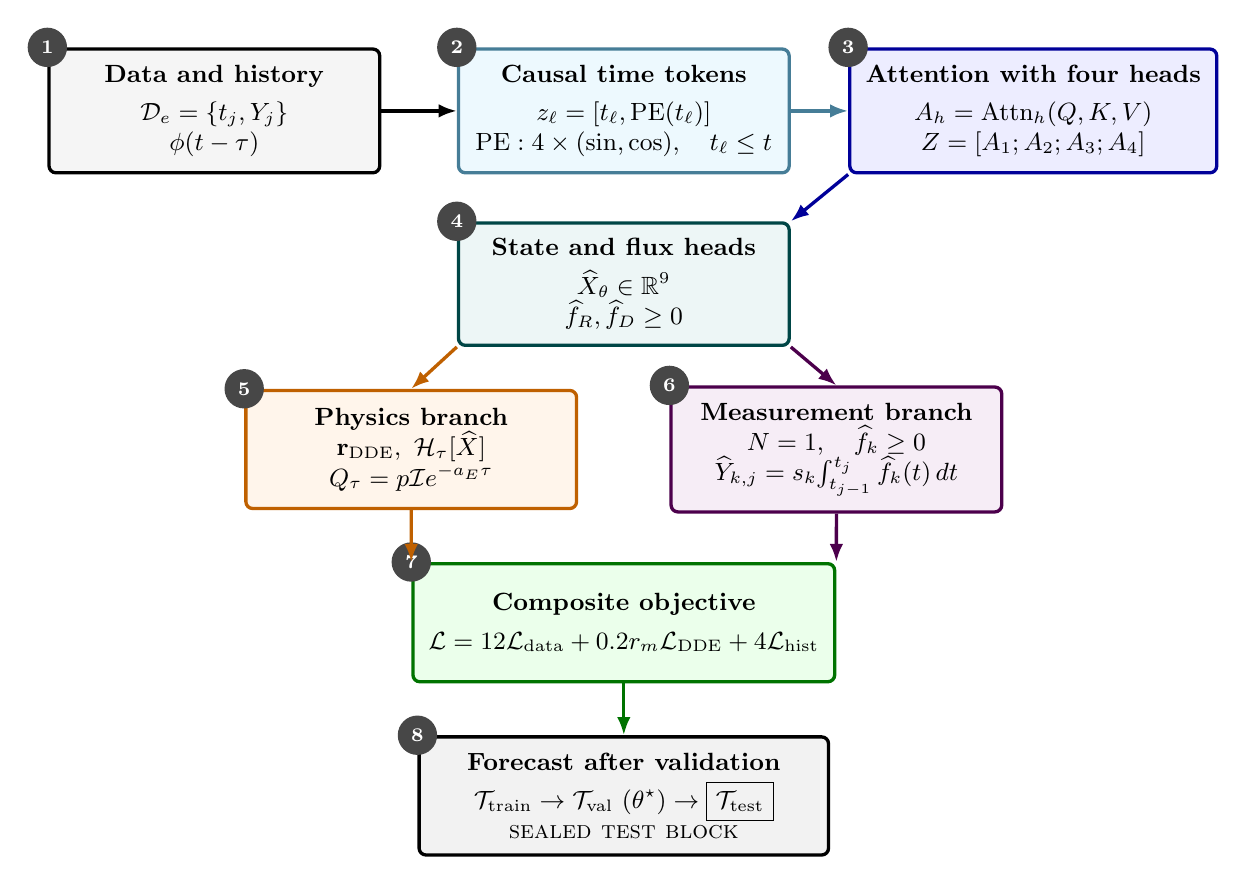
\begin{tikzpicture}[
			x=1mm,y=1mm,
			stage/.style={draw,very thick,rounded corners=2.5pt,minimum width=42mm,minimum height=15mm,align=center,inner sep=2mm,font=\small},
			branch/.style={draw,very thick,rounded corners=2.5pt,minimum width=42mm,minimum height=15mm,align=center,inner sep=2mm,font=\small},
			flow/.style={-{Latex[length=2.3mm]},very thick},
			badge/.style={circle,fill=black!72,text=white,minimum size=5mm,inner sep=0pt,font=\scriptsize\bfseries}
		]
		\node[stage,fill=gray!8] (input) at (0,0)
		{\textbf{Data and history}\\[1mm]$\mathcal D_e=\{t_j,Y_j\}$\\$\phi(t-\tau)$};
		\node[badge] at (input.north west) {1};

		\node[stage,fill=cyan!7,draw=cyan!55!black] (tokens) at (52,0)
		{\textbf{Causal time tokens}\\[1mm]$z_\ell=[t_\ell,\operatorname{PE}(t_\ell)]$\\$\operatorname{PE}:4\times(\sin,\cos),\quad t_\ell\leq t$};
		\node[badge] at (tokens.north west) {2};

		\node[stage,fill=blue!7,draw=blue!60!black] (attention) at (104,0)
		{\textbf{Attention with four heads}\\[1mm]$A_h=\operatorname{Attn}_h(Q,K,V)$\\$Z=[A_1;A_2;A_3;A_4]$};
		\node[badge] at (attention.north west) {3};

		\node[stage,fill=teal!7,draw=teal!55!black] (heads) at (52,-22)
		{\textbf{State and flux heads}\\[1mm]$\widehat X_\theta\in\mathbb R^9$\\$\widehat f_R,\widehat f_D\geq0$};
		\node[badge] at (heads.north west) {4};

		\node[branch,fill=orange!8,draw=orange!75!black] (physics) at (25,-43)
		{\textbf{Physics branch}\\$\mathbf r_{\rm DDE},\ \mathcal H_\tau[\widehat X]$\\$Q_\tau=p\mathcal I e^{-a_E\tau}$};
		\node[badge] at (physics.north west) {5};

		\node[branch,fill=violet!7,draw=violet!60!black] (measure) at (79,-43)
		{\textbf{Measurement branch}\\$N=1,\quad \widehat f_k\geq0$\\$\widehat Y_{k,j}=s_k\!\int_{t_{j-1}}^{t_j}\widehat f_k(t)\,dt$};
		\node[badge] at (measure.north west) {6};

		\node[stage,minimum width=52mm,fill=green!8,draw=green!45!black] (loss) at (52,-65)
		{\textbf{Composite objective}\\[1mm]$\mathcal L=12\mathcal L_{\rm data}+0.2r_m\mathcal L_{\rm DDE}+4\mathcal L_{\rm hist}$};
		\node[badge] at (loss.north west) {7};

		\node[stage,minimum width=52mm,fill=gray!10] (forecast) at (52,-87)
		{\textbf{Forecast after validation}\\[1mm]$\mathcal T_{\rm train}\rightarrow\mathcal T_{\rm val}\ (\theta^\star)\rightarrow\boxed{\mathcal T_{\rm test}}$\\\textsc{sealed test block}};
		\node[badge] at (forecast.north west) {8};

		\draw[flow] (input) -- (tokens);
		\draw[flow,cyan!55!black] (tokens) -- (attention);
		\draw[flow,blue!60!black] (attention.south west) -- (heads.north east);
		\draw[flow,orange!75!black] (heads.south west) -- (physics.north);
		\draw[flow,violet!60!black] (heads.south east) -- (measure.north);
		\draw[flow,orange!75!black] (physics.south) -- (loss.north west);
		\draw[flow,violet!60!black] (measure.south) -- (loss.north east);
		\draw[flow,green!45!black] (loss) -- (forecast);
		\end{tikzpicture}%
		}
		\caption{\textcolor{red}{
TransPINN workflow. Time inputs up to the query time pass through Fourier encoding and attention with four heads. The history operator supplies delayed states. State and flux outputs feed the physics and measurement branches. Both branches contribute to the common objective. Validation selects $\theta^\star$ before evaluation on the test interval. Equation~\eqref{eq:attention} defines the attention operator.
}}
		\label{fig:transpinn_workflow}
	\end{figure*}

	The available information depends on the task. In the dissertation, offline inverse simulation uses all timestamps within the observed reconstruction window. It therefore requires no autoregressive causal mask. In the rolling forecast experiment here, the query sequence is limited to $[\max(0,t-0.18),t]$. This prevents forecasts from accessing timestamps after the query time. Both settings use the scaled dot product attention in \eqref{eq:attention}. The causal restriction controls access to observations. It does not change the architecture or its physical interpretation.

	\textcolor{red}{
	We compare five implementations with the same maximum training budget. Table~\ref{tab:architecture} lists their configurations and parameter counts. Section~\ref{sec:fair_benchmark} provides an additional comparison with a Transformer trained only on data under strictly matched conditions.
	PINN uses the standard MLP solver. LSTM-PINN adapts the PhyLSTM principle~\cite{zhang2020phylstm} to the architecture used in this comparison. TimePINN applies causal weighting to the residual loss following Wang et al.~\cite{wang2024causalpinn}. We divide the residuals into eight chunks in time order. The loss is
	}

	\textcolor{red}{
	\begin{equation}
	\begin{aligned}
	\mathcal L_i&=\operatorname{MSE}(\mathbf r_i),\\
	w_i&=\exp\!\left[-2\sum_{k<i}\operatorname{stopgrad}(\mathcal L_k)\right],\\
	\mathcal L_{\rm DDE}^{\rm causal}&=\frac{1}{8}\sum_{i=1}^{8}w_i\mathcal L_i.
	\end{aligned}
	\label{eq:causal_time_loss}
	\end{equation}
	}

	\textcolor{red}{
	NoAttn-PINN has the same number of trainable parameters as TransPINN. It replaces each attention map with four linear projections applied separately to each token. Only this ablation isolates the effect of attention across tokens.
	}

	\begin{table}[t]
		\caption{\textcolor{red}{Baseline configurations. All methods use the same data, folds, DDE, history, and parameter bounds. They also share the optimization budget. The losses are identical except for the causal weighting in \eqref{eq:causal_time_loss}.}}
		\label{tab:architecture}
		\centering\footnotesize
		\begin{tabularx}{\columnwidth}{@{}lXr@{}}
		\toprule
		Method/item & Configuration & Parameters\\
		\midrule
		PINN/TimePINN & $9$--$128$--$128$--$11$ tanh MLP & 19,219\\
		LSTM-PINN & Two unidirectional layers, hidden width 36 & 17,839\\
		TransPINN & One encoder and one decoder, $d=24$, 4 heads, FFN width 48, WaveAct & 18,619\\
		NoAttn-PINN & Projections with the same parameter count, no mixing across tokens & 18,619\\
		Optimization & Adam with cosine learning rate decay from $2\times10^{-3}$. Maximum of 260 epochs. Checkpoint selection by validation. Seeds: 11, 22, 33. & --\\
		\bottomrule
		\end{tabularx}
	\end{table}


	\input{experiments/identifiability_section.tex}

	\subsection{Rolling-origin comparison and uncertainty}

	\textcolor{red}{
	For each event $e$, we find the number of bins needed to capture 99\% of the observed activity in each channel and take the larger value as $L_e$. 
	We set $h_e=\max\{2,\lfloor0.1L_e\rfloor\}$. 
	The training window starts at the first bin and initially ends at bin $\lceil0.5L_e\rceil$. 
	We then extend it by $h_e$ bins at each step. 
	The next $h_e$ bins form the validation interval, 
	and the following $h_e$ bins form the test interval. 
	We retain the first three splits with positive activity in both channels in both validation and test intervals.
	}

	\textcolor{red}{
	This rule uses the observed series to determine eligible splits before fitting and applies to all models. 
	Validation and test values are not used for normalization, gradient updates, checkpoint selection, or hyperparameter changes. 
	Table~\ref{tab:event_data} reports the resulting boundaries.
	}
	\textcolor{red}{
	This design replaces the previous 60/20/20 split of the full series. 
	Under the 60/20/20 split, the Harvey test interval contains no rumor activity. 
	For Sydney, the validation interval has no activity in either channel, 
	and the test interval contains only one rumor item and no corrective items. 
	We exclude errors from these largely inactive intervals because they provide little evidence of forecasting performance. 
	For a channel with $n$ test bins and $n_{\rm tr}$ training bins, 
	the primary metric is
	}

	\textcolor{red}{
	\begin{equation}
	\operatorname{NRMSE}=\frac{\sqrt{n^{-1}\sum_j(\widehat Y_j-Y_j)^2}}
	{\max\!\left\{1,\sqrt{n_{\rm tr}^{-1}\sum_{j\in{\rm tr}}Y_j^2}\right\}}.
	\label{eq:nrmse}
	\end{equation}
	}
	
	\textcolor{red}{
We first average results across channels within each fold. We then average across folds within each event. We report two evaluations. The first assesses robustness across seeds. For each seed, we average the event results. Table~\ref{tab:validation} reports the mean and sample standard deviation across the three seeds specified in advance.
The second evaluates performance after validation selects a seed. For each event, fold, and model, we choose the seed with the lowest validation objective. Exact ties favor the smaller seed. All methods follow this rule. Selection uses no test predictions or errors. NMAE uses the same denominator computed only from training data. Runtime measures the elapsed time for one CPU fit with a given event, fold, and seed.
}

\begin{table*}[t]
	\caption{\textcolor{red}{Robustness across all seeds. Event columns and macro NRMSE report test NRMSE as mean $\pm$ sample SD across seeds. Macro NMAE follows the same averaging procedure. Bold values indicate the lowest mean. They do not imply statistical significance.}}
	\label{tab:validation}
	\centering\scriptsize
	\setlength{\tabcolsep}{2.7pt}
	\begin{tabular}{@{}lccccccrr@{}}
	\toprule
	Method & Harvey & CSDC & Ottawa & Sydney & Macro NRMSE & Macro NMAE & Parameters & s/fit\\
	\midrule
	PINN & $0.399\!\pm\!0.019$ & $0.435\!\pm\!0.061$ & $\mathbf{0.447\!\pm\!0.113}$ & $\mathbf{0.549\!\pm\!0.060}$ & $\mathbf{0.457\!\pm\!0.052}$ & $0.395\!\pm\!0.049$ & 19,219 & 1.53\\
	LSTM-PINN & $0.561\!\pm\!0.124$ & $0.428\!\pm\!0.001$ & $0.548\!\pm\!0.012$ & $0.559\!\pm\!0.069$ & $0.524\!\pm\!0.031$ & $0.460\!\pm\!0.032$ & 17,839 & 6.31\\
	TimePINN & $0.397\!\pm\!0.022$ & $0.437\!\pm\!0.065$ & $0.451\!\pm\!0.118$ & $0.572\!\pm\!0.044$ & $0.464\!\pm\!0.050$ & $0.402\!\pm\!0.050$ & 19,219 & 1.61\\
	NoAttn-PINN & $\mathbf{0.370\!\pm\!0.046}$ & $\mathbf{0.417\!\pm\!0.019}$ & $0.574\!\pm\!0.145$ & $0.555\!\pm\!0.075$ & $0.479\!\pm\!0.044$ & $0.412\!\pm\!0.049$ & 18,619 & 13.20\\
	TransPINN & $0.453\!\pm\!0.175$ & $0.428\!\pm\!0.041$ & $0.562\!\pm\!0.171$ & $0.585\!\pm\!0.180$ & $0.507\!\pm\!0.059$ & $0.444\!\pm\!0.058$ & 18,619 & 21.58\\
	\bottomrule
	\end{tabular}
\end{table*}

\begin{figure}[t]
	\centering
	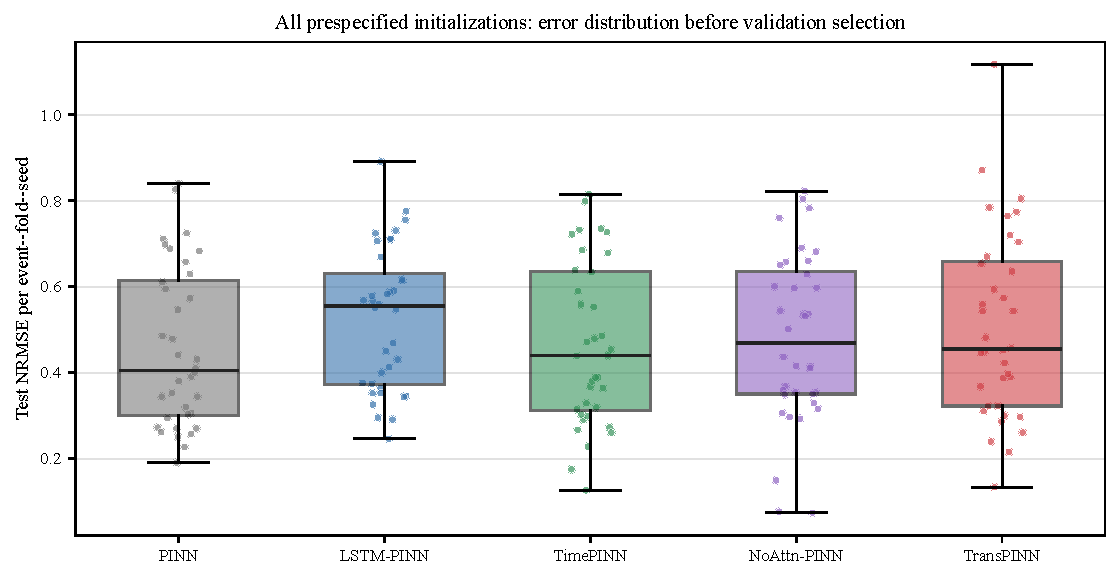
\includegraphics[width=0.98\columnwidth]{output/figures/all_seed_error_distribution.pdf}
	\caption{\textcolor{red}{Distribution of test NRMSE across 36 combinations of events, folds, and seeds for each method before validation selection. Some TransPINN runs achieve competitive errors. Its distribution also has a wider upper tail. We therefore report robustness separately from performance after selection.}}
	\label{fig:seed_distribution}
\end{figure}

Table~\ref{tab:validation_selected} reports test performance after seed selection using validation alone. Among the five methods, TransPINN has the lowest macro NRMSE and NMAE point estimates. It also has the lowest NRMSE for Harvey and CSDC. PINN leads on Ottawa. NoAttn-PINN leads on Sydney.

\begin{table*}[t]
	\caption{\textcolor{red}{Test performance after validation selects a seed. Event entries report NRMSE as mean $\pm$ sample SD across three folds. Macro NRMSE and NMAE give equal weight to each event. Selection uses the same three seeds for every method, without access to test values.}}
	\label{tab:validation_selected}
	\centering\scriptsize
	\setlength{\tabcolsep}{3.2pt}
	\begin{tabular}{@{}lcccccc@{}}
	\toprule
	Method & Harvey & CSDC & Ottawa & Sydney & Macro NRMSE & Macro NMAE\\
	\midrule
	PINN & $0.381\!\pm\!0.203$ & $0.456\!\pm\!0.321$ & $\mathbf{0.352\!\pm\!0.049}$ & $0.634\!\pm\!0.089$ & $0.456$ & $0.395$\\
	LSTM-PINN & $0.443\!\pm\!0.255$ & $0.423\!\pm\!0.127$ & $0.544\!\pm\!0.072$ & $0.584\!\pm\!0.255$ & $0.499$ & $0.432$\\
	TimePINN & $0.381\!\pm\!0.236$ & $0.457\!\pm\!0.296$ & $0.361\!\pm\!0.041$ & $0.641\!\pm\!0.091$ & $0.460$ & $0.399$\\
	NoAttn-PINN & $0.364\!\pm\!0.258$ & $0.424\!\pm\!0.074$ & $0.494\!\pm\!0.129$ & $\mathbf{0.536\!\pm\!0.164}$ & $0.455$ & $0.385$\\
	TransPINN & $\mathbf{0.348\!\pm\!0.169}$ & $\mathbf{0.411\!\pm\!0.138}$ & $0.380\!\pm\!0.064$ & $0.607\!\pm\!0.140$ & $\mathbf{0.436}$ & $\mathbf{0.366}$\\
	\bottomrule
	\end{tabular}
\end{table*}



\textcolor{red}{
We assess uncertainty in pairwise differences using 5000 deterministic replicates of a paired hierarchical bootstrap. Events form the outer clusters with equal weights. We resample folds within each event. We also use circular blocks of length $\lceil\sqrt{n}\rceil$, where $n$ is the number of test bins. Sampling consecutive bins preserves part of the temporal dependence. The same blocks apply to both methods and both channels.The same blocks apply to both methods and both channels.
The robustness analysis also resamples seeds. The analysis after validation selection keeps the chosen seed fixed for each event, fold, and model. In Table~\ref{tab:paired_bootstrap}, we define $d={\rm NRMSE}_{\rm baseline}-{\rm NRMSE}_{\rm TransPINN}$. Positive values favor TransPINN.
}


\begin{table*}[t]
	\caption{\textcolor{red}{Paired comparison with TransPINN using a hierarchical block bootstrap. Point differences after validation selection favor TransPINN. Every 95\% interval includes zero.}}
	\label{tab:paired_bootstrap}
	\centering\scriptsize
	\begin{tabular}{@{}lccccc@{}}
	\toprule
	& \multicolumn{2}{c}{Across all seeds} & \multicolumn{3}{c}{After validation selection}\\
	\cmidrule(lr){2-3}\cmidrule(lr){4-6}
	Baseline & $d$ & 95\% interval & $d$ & 95\% interval & $\Pr^*(d>0)$\\
	\midrule
	PINN & $-0.050$ & $[-0.134,0.041]$ & $0.019$ & $[-0.050,0.108]$ & 0.685\\
	LSTM-PINN & $0.017$ & $[-0.060,0.115]$ & $0.062$ & $[-0.072,0.163]$ & 0.855\\
	TimePINN & $-0.043$ & $[-0.130,0.042]$ & $0.023$ & $[-0.043,0.109]$ & 0.732\\
	NoAttn-PINN & $-0.028$ & $[-0.091,0.024]$ & $0.018$ & $[-0.091,0.103]$ & 0.680\\
	\bottomrule
	\end{tabular}
\end{table*}

\begin{figure*}[t]
	\centering
	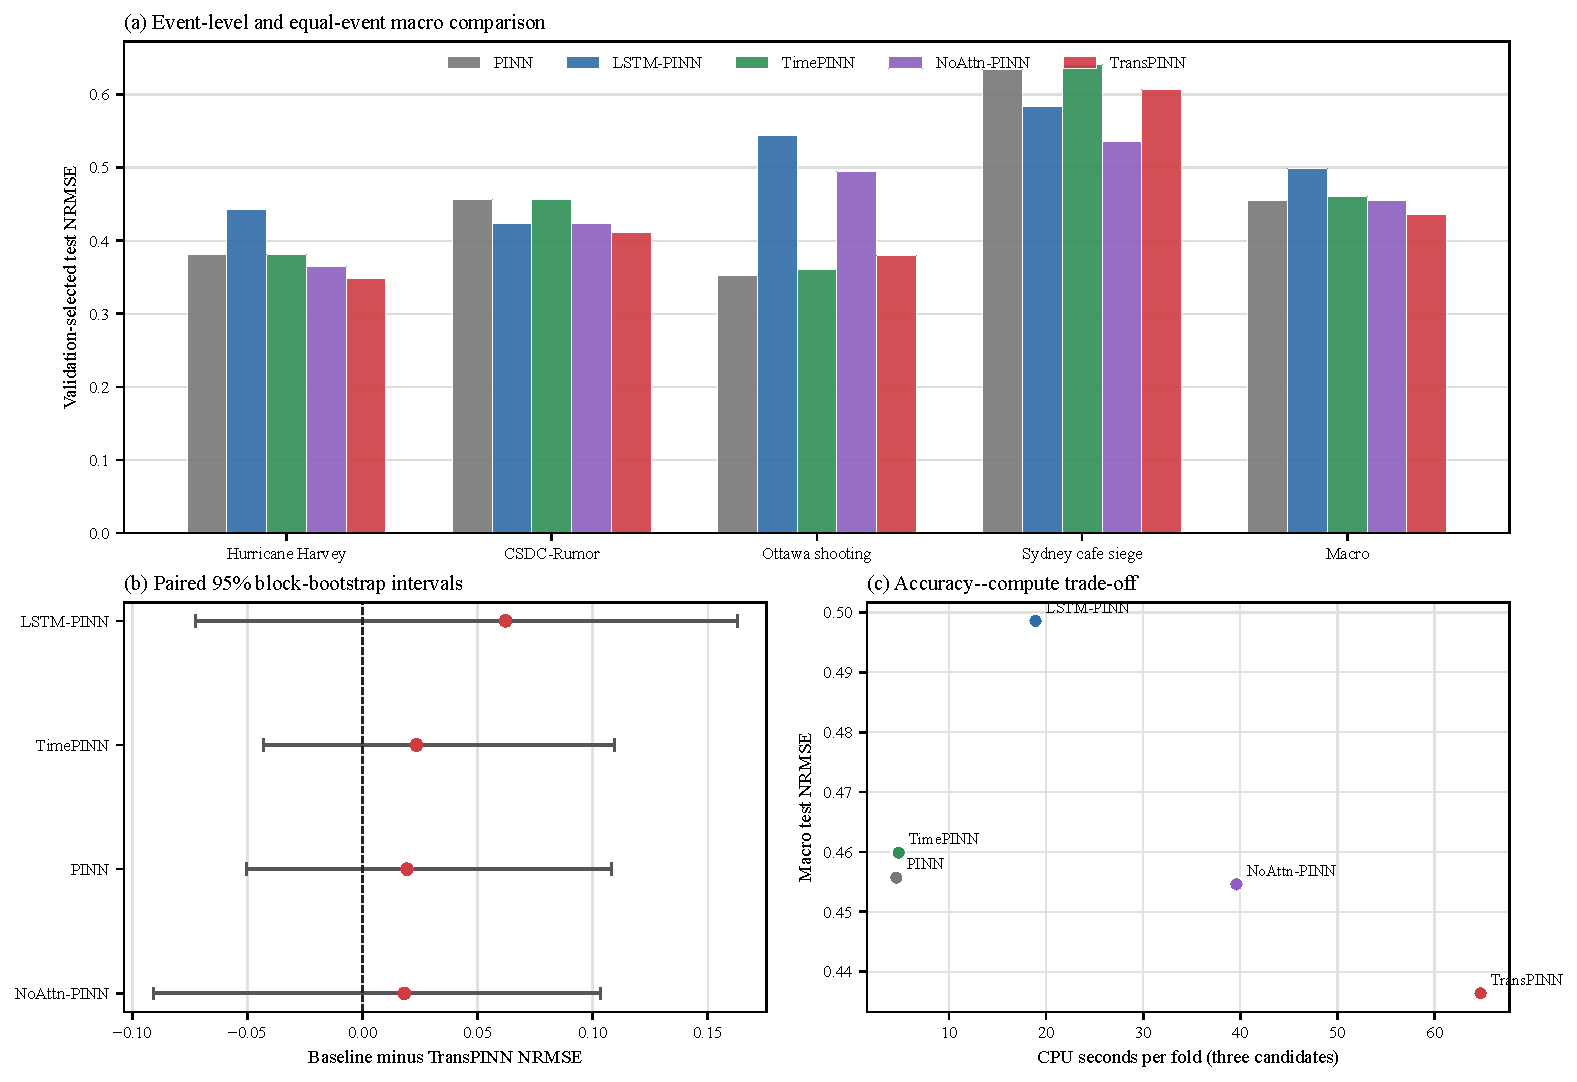
\includegraphics[width=0.98\textwidth]{output/figures/validation_selected_overview.pdf}
	\caption{\textcolor{red}{Comparison of the five methods after validation selection. (a) Event and macro NRMSE. (b) Paired NRMSE differences from the block bootstrap. Positive values favor TransPINN. (c) Accuracy and computational cost for fitting all three seed candidates. TransPINN has the lowest macro point error but the highest CPU cost. The paired intervals do not establish a clear advantage.}}
	\label{fig:selected_overview}
\end{figure*}

\begin{figure*}[t]
	\centering
	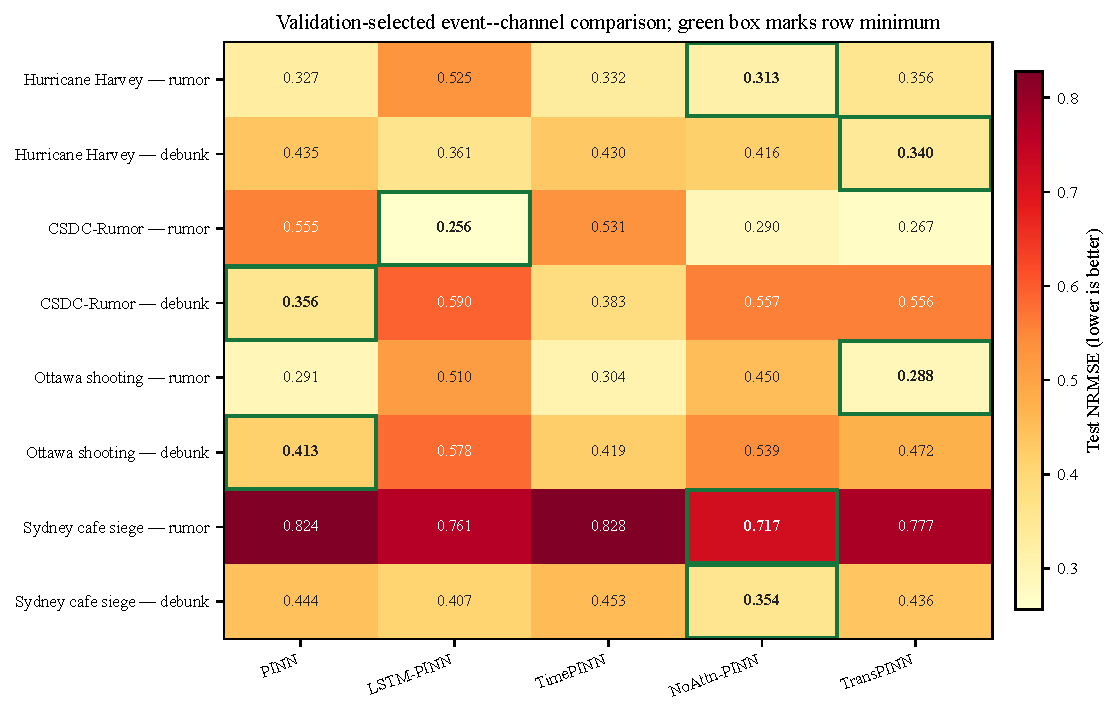
\includegraphics[width=0.88\textwidth]{output/figures/validation_selected_event_channel_heatmap.pdf}
	\caption{\textcolor{red}{Test NRMSE after validation selection, averaged across rolling folds for each event and channel. Bold green boxes mark the minimum in each row. No method leads across all events and channels.}}
	\label{fig:selected_heatmap}
\end{figure*}

\begin{figure*}[t]
	\centering
	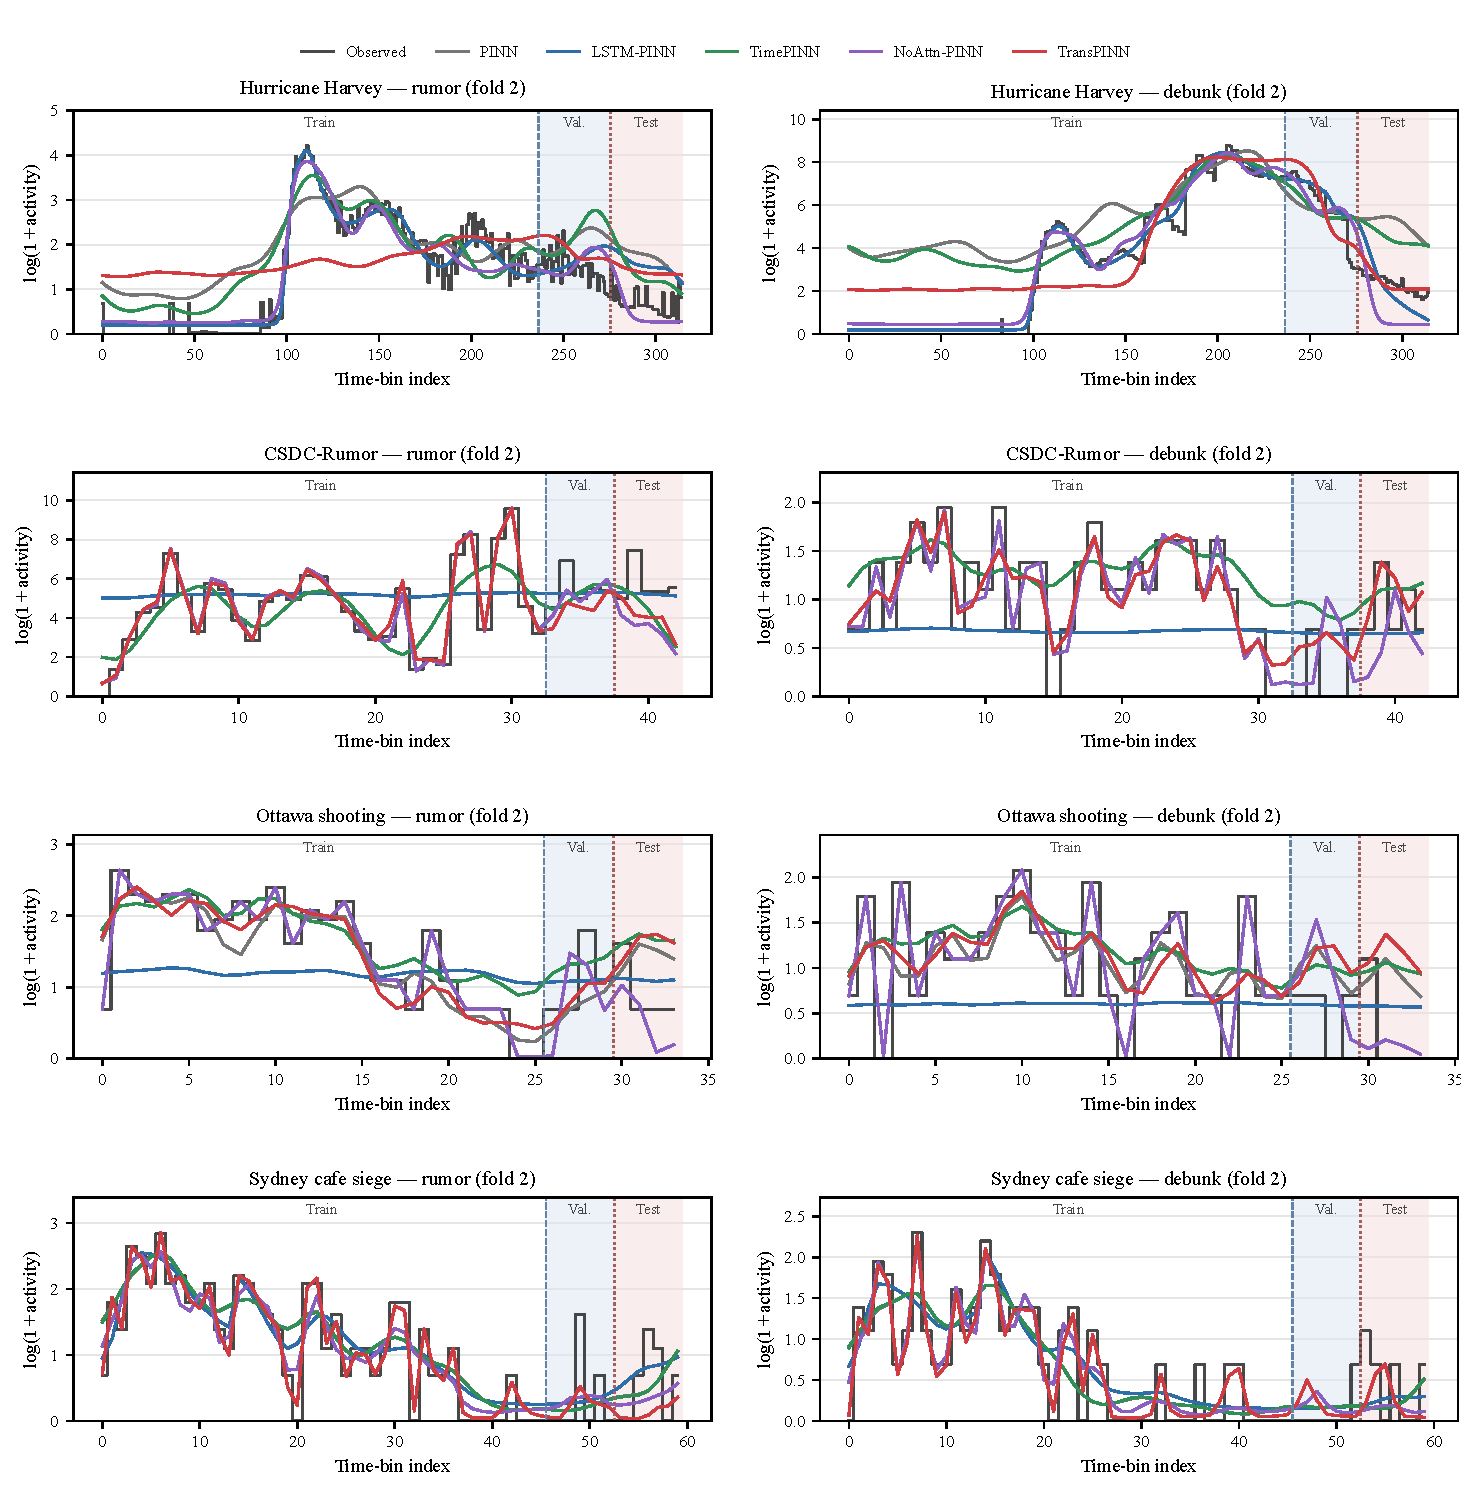
\includegraphics[width=0.98\textwidth]{output/figures/validation_selected_forecasts.pdf}
	\caption{\textcolor{red}{Predictions for the middle rolling fold of each scenario and channel on the $\log(1+\mathrm{activity})$ scale. Blue backgrounds mark validation intervals. Red backgrounds mark test intervals. Each method uses the seed chosen through validation alone. Tables~\ref{tab:validation_selected} and \ref{tab:paired_bootstrap} use all folds for statistical analysis. The curves show individual forecasts without confidence bands. They do not reproduce the dissertation's ensemble fits over the full observation window.}}
	\label{fig:multievent_forecasts}
\end{figure*}

\textcolor{red}{
The two evaluations address different questions. Across all seeds, TransPINN has a macro NRMSE of 0.507. The corresponding values are 0.524 for LSTM-PINN, 0.464 for TimePINN, 0.457 for PINN, and 0.479 for NoAttn-PINN. Figure~\ref{fig:seed_distribution} also shows a wider upper tail for TransPINN.
After validation selection, TransPINN has the lowest macro NRMSE at 0.436. The point reductions relative to LSTM-PINN, TimePINN, PINN, and NoAttn-PINN are 12.5\%, 5.1\%, 4.2\%, and 4.0\%, respectively. Against each baseline, TransPINN has a lower point error in three of the four events. The difference between NoAttn-PINN and TransPINN changes from $-0.028$ across all seeds to $+0.018$ after selection.
}

The dissertation's normalized delay sweep reports offline simulation MSE for PINN and TransPINN. Both methods use the full observation window for reconstruction. This experiment measures numerical robustness to a prescribed normalized delay $\tau$.

Tables~\ref{tab:validation}--\ref{tab:paired_bootstrap} evaluate forecasts over future intervals. They cover multiple events, folds, and seeds across five architectures. These results measure predictive performance on unseen data, both across all seeds and after validation selection. The two experiments use different information and error scales. They also measure different quantities. Their figures therefore do not represent repeated measurements of the same experiment.

\textcolor{red}{
All five methods use the same validation rule. TransPINN's lower point error comes with a higher computational cost. Fitting three TransPINN candidates takes about 64.7 CPU seconds per event and fold. PINN takes 4.6 seconds. NoAttn-PINN takes 39.6 seconds. Every paired interval in Table~\ref{tab:paired_bootstrap} includes zero.
TransPINN therefore has the lowest point error after validation selection among these five implementations. However, the four sparse cascades do not establish a statistically clear advantage or consistent gains from attention across settings. The next experiment compares models with strictly matched capacity. It also includes a baseline without physics constraints.
}

	\input{experiments/fair_benchmark_section.tex}
	\input{experiments/robustness_section.tex}
	\subsection{Ablation of cognitive fatigue and antagonistic media}
	\label{sec:mechanism_ablation}
	
	\textcolor{red}{To separate the two mechanisms from the attention architecture, we retrain TransPINN with each mechanism removed in turn. Write $F(M)=\chi/(\chi+M_1+M_2)$ for the fatigue factor in Eq.~\eqref{sys:functions}. The no-fatigue variant takes the limit $\chi\to\infty$: it sets $F=1$ in both adoption rates and $\Gamma_U=0$, removing load-dependent attenuation and fatigue-driven withdrawal together. This gives
	\begin{equation}
	\Gamma_R^{\rm NF}=\frac{q_RM_2}{1+\varpi_1M_1},\qquad
	\Gamma_D^{\rm NF}=\frac{q_DM_1}{1+\varpi_2M_2}.
	\end{equation}
	The no-antagonistic-function variant instead sets $\varpi_1=\varpi_2=0$, giving $\Gamma_R^{\rm NA}=q_RM_2F$ and $\Gamma_D^{\rm NA}=q_DM_1F$, while retaining $\Gamma_U$. This removes the competitive inhibition denominators only. Media production, the delayed pathway, and the $R\leftrightarrow D$ conversion terms remain. Thus, the comparison tests the specified antagonistic function rather than the entire media subsystem.}

	\textcolor{red}{
	All three variants use the same Transformer, observation heads, parameter bounds, loss weights, optimizer, and 260-epoch maximum budget. Each is fitted independently on the same four events, three rolling folds, and seeds 11, 22, and 33, yielding 108 fits. Parameters are re-estimated after each removal. $\chi$ is inactive in the no-fatigue variant. Checkpoints and the deployed seed are chosen using validation loss alone, as in the preceding comparison. Table~\ref{tab:mechanism_ablation} reports both the all-seed results and the validation-selected forecasts. The attention ablation remains the separate, parameter-matched comparison with NoAttn-PINN in Tables~\ref{tab:validation} and~\ref{tab:validation_selected}.
	}
	\begin{table*}[t]
	\centering
	\caption{\textcolor{red}{Separate mechanism ablations. All-seed NRMSE is the macro mean $\pm$ sample SD across three seeds. Selected metrics use the common validation-only rule. $\Delta={\rm NRMSE}_{\rm ablated}-{\rm NRMSE}_{\rm full}$. Positive values favor the full model. Intervals use 5000 paired hierarchical block-bootstrap replicates. Extra decimal places distinguish the small effects, not measurement precision.}}
	\label{tab:mechanism_ablation}
	\small
	\setlength{\tabcolsep}{5pt}
	\begin{tabular}{lccccc}
	\toprule
	Variant & All-seed NRMSE & Selected NRMSE & Selected NMAE & $\Delta$ & 95\% interval for $\Delta$\\
	\midrule
	Full TransPINN & $0.506937\pm0.058693$ & 0.436389 & 0.366302 & --- & ---\\
	Without cognitive fatigue & $0.508392\pm0.057084$ & 0.436042 & 0.366169 & $-0.000347$ & $[-0.001521,\ 0.000208]$\\
	Without antagonistic function & $0.508711\pm0.057339$ & 0.436661 & 0.366613 & $+0.000272$ & $[0.000001,\ 0.000934]$\\
	\bottomrule
	\end{tabular}
	\end{table*}

	\textcolor{red}{
		Removing fatigue slightly lowers the validation-selected NRMSE, from 0.436389 to 0.436042. Its signed contribution, $100\Delta/{\rm NRMSE}_{\rm ablated}$, is therefore $-0.080\%$, and the paired interval includes zero. Removing the antagonistic function raises NRMSE to 0.436661, corresponding to a $0.062\%$ contribution. Its interval lies just above zero, but the absolute difference is only $2.72\times10^{-4}$. Across all seeds, removing either mechanism increases mean NRMSE by less than 0.002, much less than the across-seed standard deviations. These results do not establish a consistent forecasting benefit from fatigue and show only a very small benefit from the antagonistic function under the present protocol. The mechanisms describe distinct model responses, but the two observed activity channels provide limited evidence for their individual predictive value. The comparisons do not identify causal media or fatigue effects.
	}

	\section{Optimal Control Analysis}
	\label{sec4}

	\subsection{Controls and objective}
	\textcolor{red}{
	Let $u_1$ be effort that suppresses the rumor-adoption pathway and let $u_2$ be effort that promotes the corrective pathway. This resolves the former interpretation in which a purported intervention reduced debunking. With $Z=\chi+M_1+M_2$, define the uncontrolled rates
	\begin{equation*}
	\overline\Gamma_R=\frac{q_R\chi M_2}{(1+\varpi_1M_1)Z},\qquad
	\overline\Gamma_D=\frac{q_D\chi M_1}{(1+\varpi_2M_2)Z},
	\end{equation*}
	and the controlled rates}
	\textcolor{red}{
	\begin{equation}
	\Gamma_R^u=(1-u_1)\overline\Gamma_R,\qquad
	\Gamma_D^u=(1+u_2)\overline\Gamma_D.
	\label{control_functions}
	\end{equation}}
	The admissible set is $\mathcal U=\{u_i\in L^\infty(0,t_f):0\leq u_i\leq u_{i,\max}\}$, with $u_{1,\max}<1$. The objective is
	\begin{equation}
	J(u)=\int_0^{t_f}\left(A_RR+A_EE+A_HH+\frac{B_1u_1^2+B_2u_2^2}{2}\right)dt.
	\label{obj_func}
	\end{equation}

	\subsection{Hamiltonian and complete delayed adjoint system}
	\textcolor{red}{
	Write $x=(S_u,S_e,E,H,R,D,U,M_1,M_2)^T$, }
	
	\textcolor{red}{
	\noindent
	$b=(0,0,-1,1,0,0,0,0,0)^T$, and
	$g(x)=p(M_1,M_2)\mathcal I(x)$. Then the controlled state equation has the compact form
	\begin{equation*}
	\dot x(t)=f(x(t),u(t))+b e^{-a_E\tau}g(x(t-\tau)).
	\end{equation*}
	For the running cost $\ell$ in \eqref{obj_func}, the Hamiltonian is
	\begin{equation}
	\mathscr H(t)=\ell(x,u)+W(t)^Tf(x,u)+W(t)^Tb e^{-a_E\tau}g(x_\tau).
	\label{eq:hamiltonian}
	\end{equation}
	}
	\textcolor{red}{
	For compactness, put
	$\omega_\tau(t)=\mathbf 1_{[0,t_f-\tau]}(t)e^{-a_E\tau}$.
	}

	\begin{theorem}[Existence and necessary conditions]
		An optimal control exists. For an optimal pair $(x^*,u^*)$, there is an absolutely continuous costate $W$ satisfying
		\begin{align}
		\dot W(t)={}&-\ell_x-f_x(x^*,u^*)^TW(t)\nonumber\\
		&\textcolor{red}{-\omega_\tau(t)\nabla g(x^*(t))
		[W_H(t+\tau)-W_E(t+\tau)],}
		\label{eq:adjoint_vector}\\
		W(t_f)={}&0,\qquad W(t)=0\quad(t>t_f).
		\label{eq:terminal_costate}
		\end{align}
		Together with the state equation, these nine scalar equations and the projected controls below form the complete optimality system.
	\end{theorem}
	\begin{proof}
		\textcolor{red}{The state set is bounded by Theorem~\ref{thm:positive}. The right-hand side is locally Lipschitz, the control set is nonempty, convex, and compact, the dynamics are affine in $u$, and the running cost is coercive and strictly convex in $u$. Standard existence and delayed Pontryagin arguments \cite{lenhart2007optimal,belhdid2024optimal} give \eqref{eq:adjoint_vector}--\eqref{eq:terminal_costate}. The advanced term is the derivative, at time $t+\tau$, of the cohort flux whose delayed argument is $x(t)$.}
	\end{proof}

	\enlargethispage{1\baselineskip}
	\textcolor{red}{
	For clarity, let $\Delta_R=W_R-W_H$, $\Delta_D=W_D-W_H$,
	$\Delta_U=W_U-W_H$, and
	$\Delta_\tau(t)=W_H(t+\tau)-W_E(t+\tau)$. The media components of
	\eqref{eq:adjoint_vector} are}
	\textcolor{red}{
	\begin{align}
	\dot W_{M_1}={}&\kappa_1S_u(W_{S_u}-W_{S_e})\nonumber\\
	&+\delta_1R(W_R-W_D)+d_{M_1}W_{M_1}\nonumber\\
	&-H\!\left(\Delta_R\Gamma^u_{R,M_1}
	 +\Delta_D\Gamma^u_{D,M_1}
	 +\Delta_U\Gamma_{U,M_1}\right)\nonumber\\
	&-\omega_\tau(t)g_{M_1}(t)\Delta_\tau(t),
	\label{eq:adjoint_m1}\\
	\dot W_{M_2}={}&-\kappa_2S_e(W_{S_u}-W_{S_e})\nonumber\\
	&-\delta_2D(W_R-W_D)+d_{M_2}W_{M_2}\nonumber\\
	&-H\!\left(\Delta_R\Gamma^u_{R,M_2}
	 +\Delta_D\Gamma^u_{D,M_2}
	 +\Delta_U\Gamma_{U,M_2}\right)\nonumber\\
	&-\omega_\tau(t)g_{M_2}(t)\Delta_\tau(t).
	\label{eq:adjoint_m2}
	\end{align}
	}
	\textcolor{red}{The $\Gamma_U$ terms, omitted in the former derivation, are now explicit. The delayed derivatives use the current state $x(t)$ and the future costates, not future media multiplied by future $E$.}

	\subsection{\textcolor{red}{Required derivatives and optimal controls}}
	\textcolor{red}{All fatigue and product-rule terms are retained:}
	\textcolor{red}{
	\begin{align*}
	\overline\Gamma_{R,M_1}&=-\frac{q_R\chi M_2[\varpi_1Z+(1+\varpi_1M_1)]}{(1+\varpi_1M_1)^2Z^2},\\
	\overline\Gamma_{R,M_2}&=\frac{q_R\chi(\chi+M_1)}{(1+\varpi_1M_1)Z^2},\\
	\overline\Gamma_{D,M_1}&=\frac{q_D\chi(\chi+M_2)}{(1+\varpi_2M_2)Z^2}.
	\end{align*}
	\begin{align*}
	\overline\Gamma_{D,M_2}&=-\frac{q_D\chi M_1[\varpi_2Z+(1+\varpi_2M_2)]}{(1+\varpi_2M_2)^2Z^2},\\
	\Gamma_{U,M_1}&=\Gamma_{U,M_2}=\frac{q_U\chi}{Z^2}.
	\end{align*}
	}

	\textcolor{red}{Moreover, $\Gamma^u_{R,M_i}=(1-u_1)\overline\Gamma_{R,M_i}$,
	$\Gamma^u_{D,M_i}=(1+u_2)\overline\Gamma_{D,M_i}$, and}
	\textcolor{red}{
	\begin{equation*}
	p_{M_1}=\frac{\rho M_2}{(1+\rho M_1M_2)^2},\qquad
	p_{M_2}=\frac{\rho M_1}{(1+\rho M_1M_2)^2}.
	\end{equation*}
	}
	
	\textcolor{red}{
	Thus $\nabla g=p\nabla\mathcal I+\mathcal I\nabla p$, which completely specifies the advanced term in all nine adjoints.
	}
	\textcolor{red}{
	The stationarity derivatives are}
	\textcolor{red}{
	\begin{align*}
	\mathscr H_{u_1}&=B_1u_1-H(W_R-W_H)\overline\Gamma_R,\\
	\mathscr H_{u_2}&=B_2u_2+H(W_D-W_H)\overline\Gamma_D.
	\end{align*}}
	
	\textcolor{red}{Let $\operatorname{Proj}_{[a,b]}z=\min\{b,\max\{a,z\}\}$. The optimal controls are}
	\textcolor{red}{
	\begin{align}
	u_1^*&=\operatorname{Proj}_{[0,u_{1,\max}]}
	\left(\frac{H(W_R-W_H)\overline\Gamma_R}{B_1}\right),\label{eq:u1star}\\
	u_2^*&=\operatorname{Proj}_{[0,u_{2,\max}]}
	\left(\frac{H(W_H-W_D)\overline\Gamma_D}{B_2}\right).
	\label{eq:u2star}
	\end{align}}
	\textcolor{red}{Both expressions include the fatigue factor through $\overline\Gamma_R,\overline\Gamma_D$.}

	\subsection{\textcolor{red}{Numerical solution and limits of the evidence}}

A reproducible numerical solution requires four steps. First, solve the state DDE using the method of steps with the specified history. Second, integrate \eqref{eq:adjoint_vector} backward using \eqref{eq:terminal_costate}. Third, update the controls through \eqref{eq:u1star}--\eqref{eq:u2star} with relaxation. Repeat these steps until the relative change in the supremum norm falls below $10^{-6}$ for states, costates, and controls.

The report must specify $A_R,A_E,A_H,B_i,u_{i,\max}$. It must also provide the DDE solver tolerances, time grid, and iteration count. Objective values must cover three cases: no control, constant control, and optimal control. A sensitivity analysis must assess the effect of $B_i$.

\textcolor{red}{
The earlier control figure relies on the former model with delayed stocks and incomplete derivatives. It therefore provides no valid evidence for the corrected system. Numerical policy conclusions require a new figure based on the corrected optimality system.
}

Small values of $B_i$ can keep controls at their upper bounds for most of the time horizon. This behavior alone does not establish the need for intervention at the maximum level.

	\section{Conclusions}
	\label{sec5}
	
	This study develops a framework for rumor propagation under information delays and cognitive overload. The model separates information reception from active cognitive processing. It combines competing media influences, Holling-II fatigue, and a survival-weighted exposure cohort to describe delayed behavioral transitions.

	From a theoretical perspective, we establish well-posedness, positivity, and boundedness under compatible histories. 
	\textcolor{red}{We derive the delay-dependent threshold $\mathcal R_0(\tau)$ and conditions for local stability and Hopf bifurcation. Delays affect both exposure duration and survival into active processing.} 
	\textcolor{red}{Their effect on stability therefore depends on the model parameters, and transient rebounds alone do not establish a Hopf bifurcation.}

	Methodologically, TransPINN combines Transformer attention with physics-informed learning to estimate rumor dynamics from sparse observations. An observation model links state transitions to recorded activity. Across four events, TransPINN achieves the lowest NRMSE of 0.436, compared with 0.455--0.499 for the baselines. However, paired comparison intervals include zero, and mechanism ablations show limited forecasting gains. Identifiability analysis also reveals media-scale ambiguity and weak parameter constraints, so inference remains conditional on fixed assumptions.

	\textcolor{red}{Regarding intervention strategies, we derive optimal-control conditions that balance rumor suppression and corrective promotion against intervention costs. The formulation accounts for fatigue and delayed effects. Numerical validation remains necessary to assess the resulting policies.}

	In summary, this framework connects rumor dynamics, data-driven forecasting, and intervention design. Future work aims to incorporate network structure, distributed delays, and platform effects, and to validate inference and control with richer data.

	\section*{Data and Code Availability}
	\textcolor{red}{The source code is available at \url{https://github.com/DavidJamesBen/model}. The accompanying revision package includes processed data, model settings, random seeds, fitted checkpoints, predictions, and instructions to reproduce the reported analyses and figures. Supplementary Material contains the full identifiability analysis and parameter tables. The original CSDC-Rumor and RumourEval data remain subject to their source terms. The Harvey aggregation has no tweet-level provenance, as disclosed in Section~\ref{sec3}.}

	\section*{Acknowledgments}
	This work was supported by the National Natural Science Foundation of China (NSFC) under Project No. 62473115 and the Fundamental Research Plan of Shenzhen Government under Project No. JCYJ20240813105202004.
	
	\bibliographystyle{IEEEtran}
	\bibliography{bib}
	
	
	\begin{IEEEbiography}
		[{\includegraphics[width=1in,height=1.25in,clip,keepaspectratio]{AUTHOR_Deliang_Li.jpg}}]{Deliang Li}
		received the B.S. degree from South China Normal University, Guangzhou, China, and is working toward the Ph.D. degree at Harbin Institute of Technology, Shenzhen, China.
		His research interests include deep-learning model design and analysis, biomathematics, ordinary differential equations, and physics-informed neural networks.
	\end{IEEEbiography}
	
	\begin{IEEEbiography}
		[{\includegraphics[width=1in,height=1.25in,clip,keepaspectratio]{AUTHOR_Yi_Zhao.jpg}}]{Yi Zhao}
		received the Ph.D. degree from Hong Kong Polytechnic University, Hong Kong, China, in 2007. Since graduating, he has been with the Harbin Institute of Technology, Shenzhen, China, and is currently a Professor. His research interests include nonlinear dynamics, nonlinear time series analysis, and complex system modeling. His recent works have been on the application of mathematical methods to a diverse range of application problems.
	\end{IEEEbiography}
	
	
	
	\begin{IEEEbiography}
		[{\includegraphics[width=1in,height=1.25in,clip,keepaspectratio]{AUTHOR_Yifeng_Wang.jpg}}]{Yifeng Wang}
		received the Ph.D. degree from Harbin Institute of Technology, Shenzhen, China. He is currently a postdoctoral researcher at Tsinghua University.
		His research interests include deep learning model design and analysis, inertial navigation, motion tracking, human activity recognition, and time series analysis.
	\end{IEEEbiography}
\end{document}
